\chapter{Dynamic Prediction of the Landmark Survival Time in Cancer Clinical Trials Using Joint Modeling Framework}
\label{chpt:chpt3}

\section{Introduction}
In recent years, many cancer drugs have received regulatory approvals based on \ac{PFS} as the primary endpoint. Although \ac{PFS} is a well-accepted surrogate endpoint for \ac{OS} in many cancer types, improvement in survival remains the clinical gold standard for assessing a patient's benefit \citep{tang2007surrogate, driscoll2009overall, methy2010surrogate, grigore2020surrogate}. However, planning a statistically well-powered \ac{OS} analysis in practice often presents challenges due to longer survival times in early-stage cancers, patients switching to alternative treatments after progression, starting other anti-cancer therapies, or being lost to follow-up. The timing of the primary analysis for trials with \ac{PFS} as the primary endpoint is determined by the number of patients progressed, and survival data is often not mature enough for meaningful statistical inference due to a low number of deaths. Hence, if \ac{PFS} is statistically significant in the final analysis, regulatory agencies often request one or more updated \ac{OS} analyses once the survival data are more mature. Updated \ac{OS} analyses are crucial for market access and reimbursement decisions. Therefore, proper planning is essential to ascertain when mature \ac{OS} data will be available.

Model-based prediction of survival time for trial participants aids research teams in efficiently allocating resources, accurately planning future \ac{OS} analyses, and understanding the potential survival benefit of an experimental drug. It also assists in designing and committing to Phase 3 trials based on disease progression data observed in Phase 2 studies. Moreover, it helps clinicians and scientists understand the mechanism of a new compound that improves patients' survival while reducing disease burden. Besides drug development, mature \ac{OS} data are crucial for decision-making by both patients and clinicians, and understanding a drug's cost-effectiveness. \cite{sborov2019impact} demonstrated that when oncologists inaccurately predict \ac{OS}, patients with advanced cancer are more likely to receive aggressive end-of-life care, often contradicting the patients' wishes. \cite{mackillop1997measuring} stated that accurate \ac{OS} prediction facilitates the effective use of limited healthcare resources and helps patients make suitable plans for their remaining lives. \cite{henderson2001accuracy} further provides examples of how accurate survival predictions have financial implications for insurance programs and health authorities.

\ac{PFS} is defined as the time from randomization until \ac{PD} or death from any cause. In oncology studies, progression is evaluated using the \ac{RECIST} \citep{eisenhauer2009new}. \ac{RECIST} provides standardized definitions and procedures for documenting how subjects progress, respond, or remain stable in terms of their disease burden during a treatment course. \ac{RECIST} offers methods for assessing solid tumor responses using X-ray, CT, and MRI scans and is recommended by the National Cancer Institute. Note, \ac{PFS} is viewed as a composite outcome with four components: 1) measurement of the target lesion, which is captured as longitudinal continuous data, 2) time to non-target lesion progression, 3) time until the emergence of a new lesion, and 4) time to death from any cause. Depending on the cancer type, each of these components has a different degree of predictivity for \ac{OS}. For example, \cite{stein2013survival} showed that the progression of non-target lesions or the appearance of new lesions is more predictive of \ac{OS} benefit than the sum of the longest tumor diameters of the target lesions for patients with metastatic renal cell carcinoma. The current practice of \ac{OS} prediction often overlooks the disease progression process and models only the number of deaths.

In this manuscript, we evaluated several model-based approaches to forecast the death times of trial participants ``still alive", leveraging information about disease progression along with important baseline factors. The relationship between \ac{PFS} and \ac{OS} has garnered interest in both statistical and clinical literature over time. Notably, \cite{fleischer2009statistical} employed exponential time-to-event distributions to describe the dependency structure between \ac{OS} and \ac{PFS}. This is further expanded by \cite{weber2019quantifying, fu2013joint, meller2019joint} by utilizing copula and multi-state models to jointly analyze \ac{PFS} and \ac{OS} without strict parametric assumptions for the marginal survival distributions of \ac{PFS} and \ac{OS}. Another important work by \cite{shukuya2016relationship} investigated the correlation between median \ac{PFS} and median \ac{OS}, concluding that both tumor response and \ac{PFS} are significant predictors of \ac{OS}. Other methodologies for \ac{OS} prediction include joint modeling of longitudinal tumor size data of the target tumor and survival data (\cite{claret2009model, claret2013evaluation, wang2009elucidation, bruno2014evaluation, zecchin2016models, lim2019predicting}), which incorporates baseline survival data into the \ac{OS} prediction. Meanwhile, \cite{yu2020new} jointly modeled the dynamics of target lesions and the progression of non-target lesions to predict \ac{PFS}. However, most of the literature in this area focuses primarily on improving the estimation of \ac{OS} rather than predicting the future survival time of patients ongoing in the trial. Moreover, to our current knowledge, there is no existing methodology that formally combines all three components of disease progression, i.e., target lesion, non-target lesion and new lesion. In this paper, we propose a joint modeling framework to address these gaps and further enhance the copula model and the multi-state model for predicting the survival times of ongoing patients.

The rest of the paper is structured as follows: A motivating example from a Phase 3 renal cell carcinoma study is used to establish the problem in Section \ref{sec:example}. This is followed by a set of proposed models that explore the correlation between disease progression and survival as presented in Section \ref{sec:method}. The simulation studies conducted to test the properties of our method are presented in Section \ref{sec:simulation}. The renal cell carcinoma example is revisited in Section \ref{sec:caseanalysis} to illustrate the practical utility of the proposed methodology. Finally, we conclude with a discussion that summarizes the key messages and lessons learned.

\section{Motivating Example: Phase 3 Study in Renal Cell Carcinoma} \label{sec:example}
The methods outlined in this paper are inspired by a phase 3, randomized, open-label, parallel-arm study. A total of 800 treatment-naive adult participants with advanced renal cell carcinoma were randomized (1:1) to receive either the experimental drug or the standard of care. A key inclusion criterion was the presence of at least one measurable lesion, as defined by \ac{RECIST} version 1.1, which had not been previously irradiated. Tumor assessments were performed using computed tomography or magnetic resonance imaging at baseline, every six weeks post-randomization for the first 18 months, and subsequently every 12 weeks until confirmed disease progression. Important baseline demographic and disease characteristics were evenly distributed between the two treatment groups. The study had two primary endpoints: \ac{PFS} and \ac{OS} among patients with programmed death ligand 1 (PD-L1)–positive tumors. The primary analysis was scheduled when at least 397 \ac{PFS} events occurred (Figure \ref{fig:evolution}). At the time of the primary \ac{PFS} analysis only 146 deaths were observed which was immature to draw any reasonable conclusion for OS. Therefore, an updated analysis of \ac{OS} was planned after 341 deaths. The trial findings indicated that patients administered the experimental drug experienced a notably extended \ac{PFS} compared to those given the standard of care. It is crucial to note that while we have utilized the data structure from a real-life trial, the actual values presented here are simulated based on published summary statistics, both for proprietary considerations and to ensure proper protection of patient data.

\begin{figure}
    \centering
    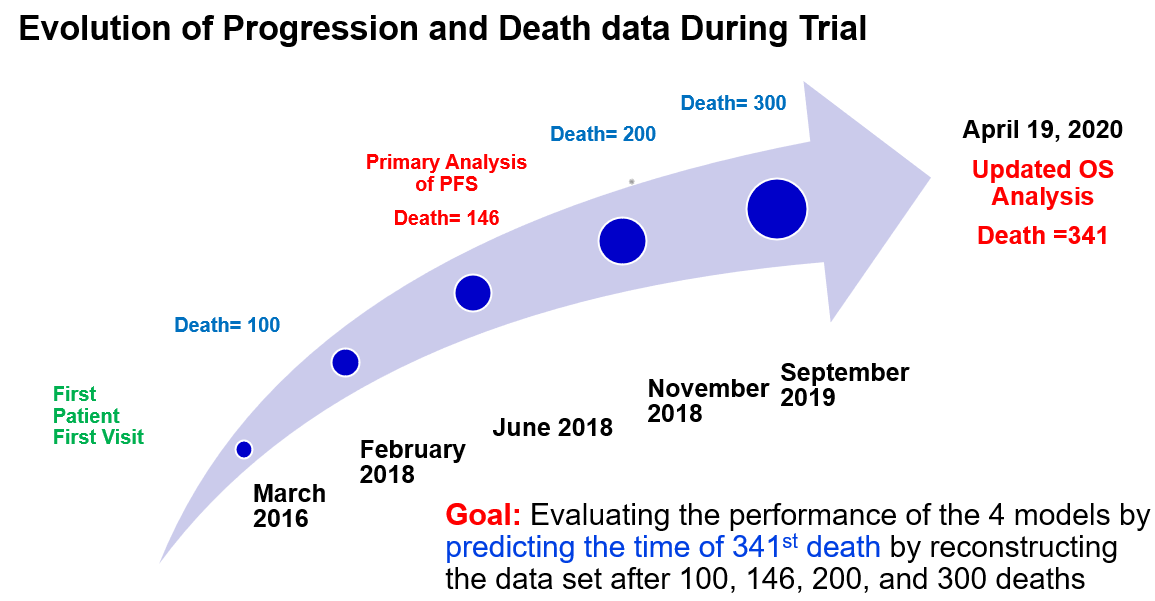
\includegraphics[width=0.85\textwidth]{chapters/figures/Evolution.png}
    \caption{Evolution of progression and death data during trial\label{fig:evolution}}
\end{figure}


We aim to use the observed data to construct a predictive tool that provides a reliable estimate of the time of the $n$th death in the trial. Specifically, we utilize data on participants' baseline characteristics, treatment group, \ac{OS}, and the processes underlying \ac{PFS}, including measurements of target lesions and the progression of disease in non-target and new lesions. This approach is justified as \ac{PFS} is known to be a strong predictor of \ac{OS} in advanced renal cell carcinoma \citep{heng2011progression}

Figure \ref{fig:profile_LD} demonstrates significant variability among individuals in the sum of the longest diameters of target lesions, making it difficult to draw any conclusions about the treatment without systematic modeling of this variability. Moreover, Kaplan-Meier plots for non-target lesions and new lesions are shown in Figures \ref{fig:NT_KMplot} and \ref{fig:NL_KMplot}, respectively. From both plots, we observe differences between the two treatment arms: patients who received the experimental drug exhibited a longer time to \ac{PD} when considering assessments of non-target lesions and new lesions. A similar trend is also observed in the Kaplan-Meier plots for \ac{OS} (Figure \ref{fig:OS_KMplot}) and \ac{PFS} (Figure \ref{fig:PFS_KMplot})

\begin{figure}
    \centering
    \subfloat[]{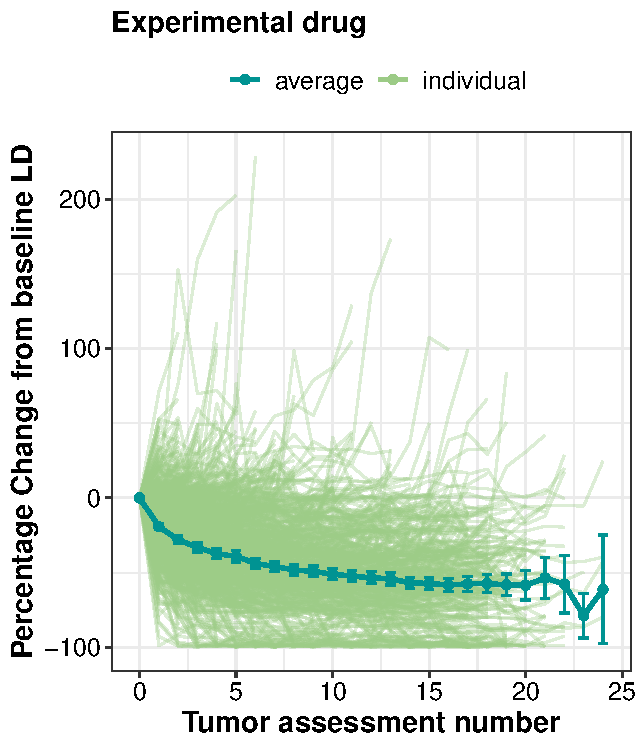
\includegraphics[width=0.45\textwidth]{chapters/figures/profile_LD_exp.pdf}\label{fig:profile_LD_exp}}
    \hfill
    \subfloat[]{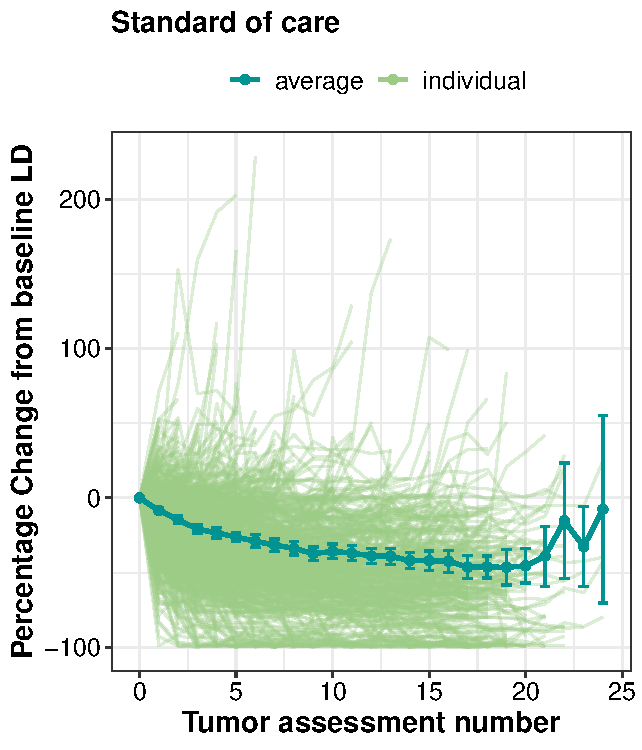
\includegraphics[width=0.45\textwidth]{chapters/figures/profile_LD_soc.pdf}\label{fig:profile_LD_soc}}
    \caption{Profile plot of the sum of the longest diameter of target lesions}
    \label{fig:profile_LD}
\end{figure}

\begin{figure}
    \centering
    \subfloat[]{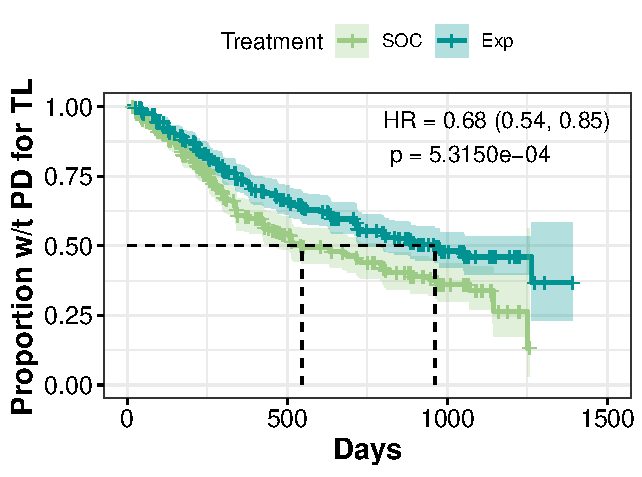
\includegraphics[width=0.45\textwidth]{chapters/figures/TL_KMplot.pdf}\label{fig:TL_KMplot}}
    \subfloat[]{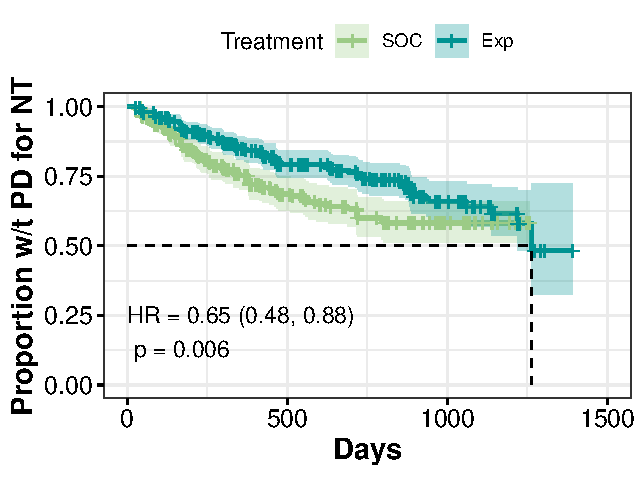
\includegraphics[width=0.45\textwidth]{chapters/figures/NT_KMplot.pdf}\label{fig:NT_KMplot}}
    \hfill
    \subfloat[]{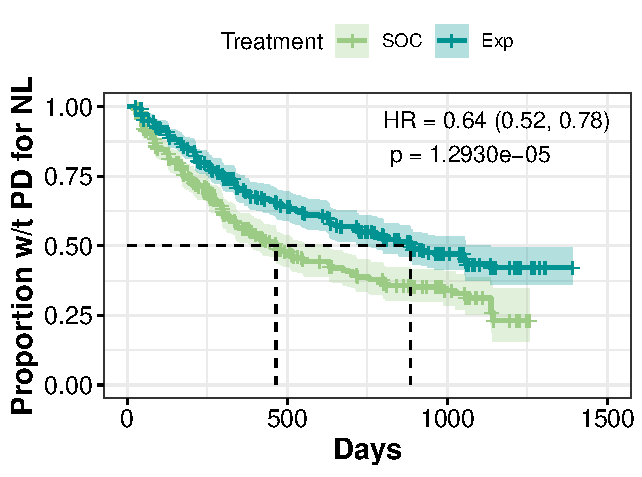
\includegraphics[width=0.45\textwidth]{chapters/figures/NL_KMplot.pdf}\label{fig:NL_KMplot}}
    \subfloat[]{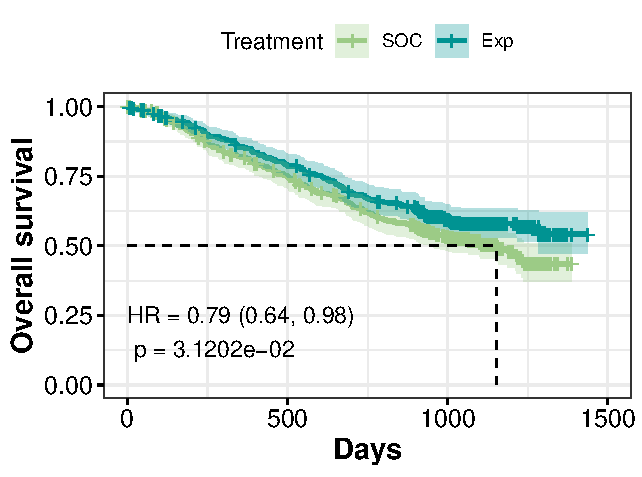
\includegraphics[width=0.45\textwidth]{chapters/figures/OS_KMplot.pdf}\label{fig:OS_KMplot}}
    \hfill
    \subfloat[]{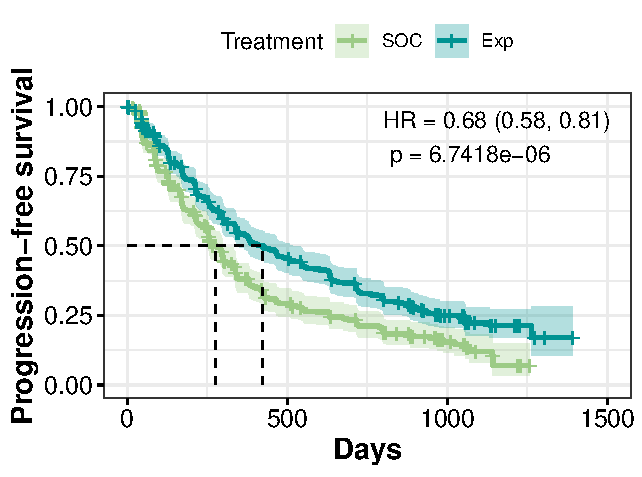
\includegraphics[width=0.45\textwidth]{chapters/figures/PFS_KMplot.pdf}\label{fig:PFS_KMplot}}
    \caption{Kaplan-Meier plots of time to progressive disease at the time of updated OS analysis considering target lesions (a), non-target lesions (b), new lesions (c), time to progressive design considering overall survival (d), and progression-free survival (e).}
\end{figure}


\section{Method}
\label{sec:method}
In this manuscript, the general process of using Bayesian statistical models to generate \ac{OS} predictions is as follows: At any given point during the clinical trial, we collect the current data and input it into our Bayesian models. Subsequently, a Markov chain Monte Carlo (MCMC) process is utilized to estimate the parameters. These estimations are then used to generate predicted \ac{OS} outcomes by leveraging the posterior predictive distribution (PPD) technique. This process allows us to create a predictive framework that is both dynamic and reflective of the evolving nature of trial data, providing timely and robust predictions for OS.


\subsection{Bayesian Model-Averaged Joint Modeling Approach}
\label{sec:jm}

In this section, we outline our proposed model by establishing three distinct joint models between each of the processes of disease progression and OS. These three joint models include the joint model between the sum of the longest diameter of target lesions and OS, the joint model between the time to non-target lesion \ac{PD} and OS, and the joint model between the time to new lesion \ac{PD} and OS. Furthermore, we incorporate a marginal model directly modeling OS. Three main steps are included in our model. First, we mitigate ``information loss" by considering all four granular components of PFS. By constructing joint, marginal models for each component, we derive real-time \ac{OS} predictions from each trial participants ``still alive". This results in four sets of intermediate predictions. Second, our proposed methods fully encapsulate the association between progression and death by incorporating random processes. Third, we enhance the accuracy of \ac{OS} predictions from \ac{PFS} by deriving the final \ac{OS} prediction from all four models' intermediate predictions simultaneously using \ac{BMA} \citep{hoeting1999bayesian}. Using the \ac{BMA} technique, we blend these different predictions to create a final predicted OS, which combines all four individual forecasts with appropriate weights. Thus, joint modeling represents a promising scientific approach to overcoming the challenges associated with \ac{OS} prediction, in comparison to existing methods that will be discussed in the subsequent sections. The structure of the proposed multivariate joint modeling approach is illustrated in Figure \ref{fig:JM}, with details provided in the following subsections.
\subsubsection{Joint Model for the Association between Target Lesion and OS} \label{sec:TL}


\begin{figure}
\centering
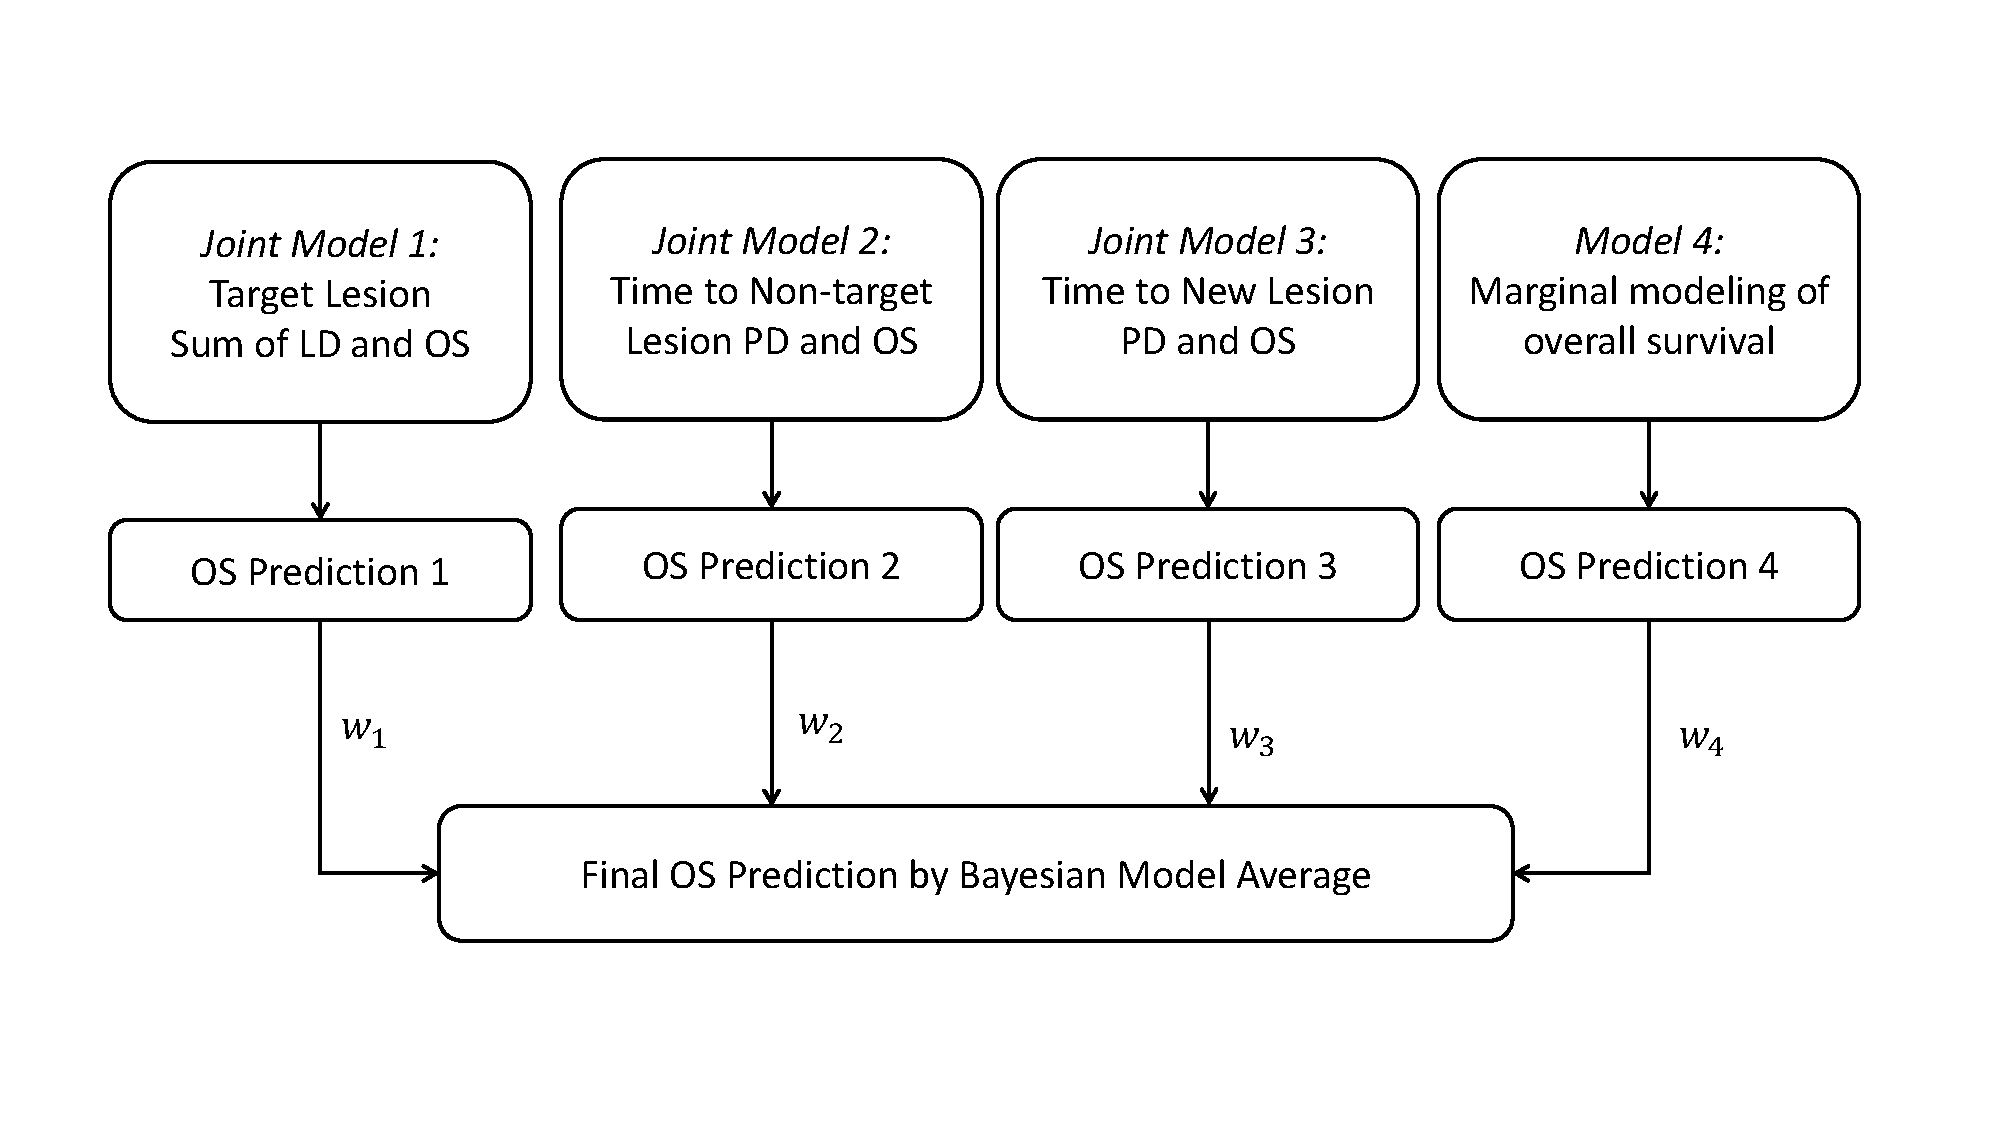
\includegraphics[width=\textwidth]{chapters/figures/JM.pdf}
%\\
%\subfloat[]{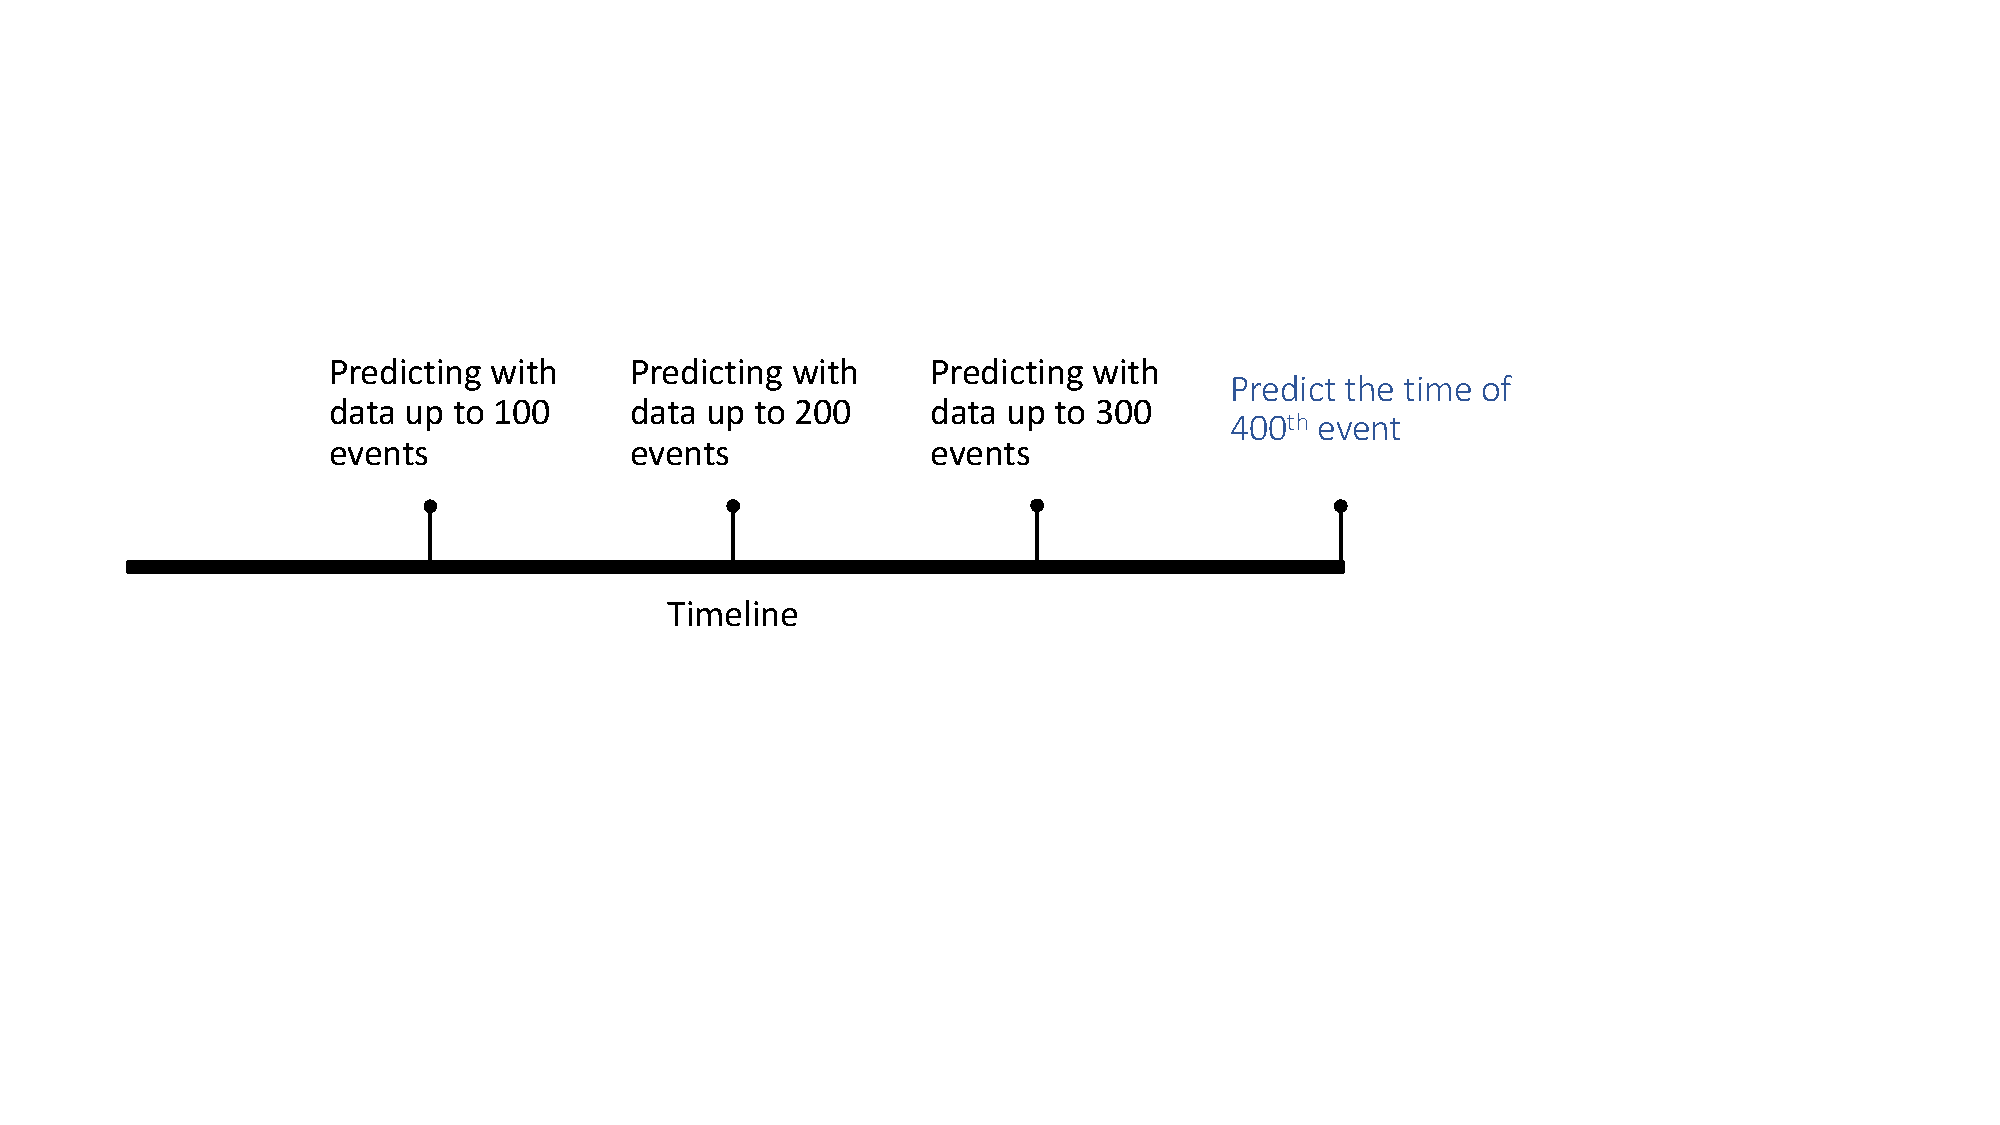
\includegraphics[width=\textwidth]{img/timeline.pdf}\label{fig:timeline}}
\caption{Multivariate joint modeling structure.} 
%(b) Predict the time of last (400th) event with observed data up to 100/200/300 events.}
\label{fig:JM}
\end{figure}


We consider a set of $n$ subjects followed over an interval of time [0,$\tau$]. Let $z_{ij}$ be the target lesion measurement (or \% change from baseline) at time $t_{ij}$ (for the $i$-th participant at the $j$-th visit), where $i=1,...,n$ and $j=1,...,k_i$. We assume the target lesion measurement time $t_{ij}$ is non-informative so that it is independent of the longitudinal measurement and event-time processes for OS. We define a latent zero-mean Gaussian process $W_i(t)$ for the $i$-th participant, independent of different participants. The following sub-models link the joint model of lesion measurements and OS:

The observed lesion measurement
$Y_{i}(t)=\mu_{i}(t)+\epsilon_i$,
where $\epsilon_i$ is the measurement error, and the lesion measurement process $\mu_{i1}$, $\mu_{i2}$,...
is modeled by the linear model
$\mu_{i}(t)=\textbf{X}_i(t)' \boldsymbol{\beta}_{\mu}+W_{i}(t)$. Here, $\textbf{X}_i(t)$ is the time-dependent covariate matrix for subject $i$'s lesion measurement. $W_i(t)$ is a Gaussian process that has the form $W_{1i}(t)=b_{1i}+b_{2i}t$,
where ($b_{1i},b_{2i}$) are zero-mean bivariate Gaussian variables with variances $\sigma_1^2$ and $\sigma_2^2$ respectively, and correlation coefficient $\rho$. 

The \ac{OS} process at time t is modeled by
$\lambda(t)=\lambda_0(t) \exp(\textbf{Z}_i' \boldsymbol{\beta}_{\rm OS}+\lambda \mu_{i}(t)+b_{3i})$.
Under a Weibull baseline hazard, $\lambda(t)$ has the form
$\lambda(t)=\alpha_{\rm OS,TL} \gamma_{\rm OS} t^{\alpha_{\rm OS,TL}-1} \exp(\textbf{Z}_i' \boldsymbol{\beta}_{\rm OS}+\lambda \mu_{i}(t)+b_{3i})$,
where $\textbf{Z}_i$ is the covariate matrix for OS, $\gamma_{\rm OS}$ and $\alpha_{\rm OS,TL}$ are the scale and shape parameters
of the Weibull distribution, and $b_{3i}\sim N(0,{\sigma_3})^2$ are random effects orthogonal to the measurement process. The construction of the likelihood for this joint model is detailed below:

The marginal distribution of the observed measurements $\mu$ is easily obtained. The likelihood for the observed data can be factorized as the product of this marginal distribution and the conditional distribution of OS, given the observed values of $\mu$. Let $\boldsymbol{\theta}_1$ denote the combined vector of unknown parameters. Conditional on lesion measurements $\mu$, OS is independent of these measurements $\mu$, so we can write the likelihood $L=L(\boldsymbol{\theta}_1, \mu, OS)$ as
$L=L_{\mu}(\boldsymbol{\theta}_1,\mu)  \times L_{OS| \mu}(\boldsymbol{\theta}_1,OS|\mu)
$,
where $L_{\mu}(\boldsymbol{\theta}_1,\mu)$ is of standard form corresponding to the marginal multivariate normal distribution of $\mu$ and
$$
L_{OS|\mu}(\boldsymbol{\theta}_1, OS|\mu)=\prod_i \bigg\{ \bigg[\lambda_0 (t) \exp(\textbf{Z}_i' \boldsymbol{\beta}_{\rm OS}+\lambda \mu_{i}(t)) \bigg]^{\delta_{OS,i}} 
$$
$$\times \exp \bigg[ -\int_0^{y_{OS,i}} \lambda_0(t) \exp(\textbf{Z}_i' \boldsymbol{\beta}_{\rm OS}+\lambda \mu_{i}(t))dt\bigg]\bigg\},
$$
here, $y_{OS,i}=\min(t_{OS,i},c_{OS,i})$ and $\delta_{OS,i}=I(t_{OS,i}\leq c_{OS,i})$. $c_{OS,i}$ is the censoring time for the $i$th participant and $t_{OS,i}$ is the true event time.


\subsubsection{Joint Model for the Association between Time to Non-Target Lesion and OS} \label{sec:NT}
Copulas are commonly used for modeling the dependence between random variables. They are continuous multivariate cumulative distributions with each random variable following a uniform marginal distribution on the interval $[0, 1]$.
Sklar's theorem states that any multivariate joint distribution can be written using univariate marginal distribution functions and a copula describing the variables' dependence structure \citep{sklar1959fonctions}. Therefore, copulas can be used to model the dependence between these survival times, allowing for more accurate prognostic prediction.
Here, we can use the copula to jointly model time to non-target lesion and OS, where time to non-target lesion corresponds to the time between randomization and \ac{PD} is observed under non-target lesion. A bivariate copula function $C:[0, 1]^2 \rightarrow [0, 1]$ of the endpoints (T, O), where $T:=$ \textit{time to non-target lesion} and $O:= OS$, can be expressed by joint survival function $\boldsymbol{S}(t, o) = T(T \geq t, O \geq o) = C(\boldsymbol{S}_{T}(t), \boldsymbol{S}_{O}(o)),$
where  $t,o \geq 0$, $\boldsymbol{S}_T$ and $\boldsymbol{S}_O$ are the marginal survival functions of $T$ and $O$, respectively \citep{weber2020statistical}. To capture various dependency patterns, one can employ different copula families. Here, we opt for the Clayton copula function \citep{clayton1978model}, which belongs to the Archimedean copula class and can capture strong dependence in the left tail. By doing so, we can express the relationship between time to non-target lesion and \ac{OS} using a single parameter $\eta_{NT}$, a parameter that can be directly linked to Kendall's tau, effectively characterizing their dependence. In the subsequent paragraphs, we formally define the copula model between time to non-target lesion and OS.

Let $t_{NT}$ and $t_{OS}$ denote times to non-target lesion and death (OS), respectively, and let $\textbf{Z}$ be covariates of interest.
For a participant with covariates $\textbf{Z}$, let $\lambda_{\rm NT}(t|\textbf{Z})$
denote the hazard function for the time to non-target lesion. Under the Cox
proportional hazards model, we have $\lambda_{\rm NT}(t_{NT}|\textbf{Z})=\lambda_{0, \rm NT}(t_{NT})\mathrm{exp}(\textbf{Z}' \boldsymbol{\beta_{\rm NT}})$.
When the baseline hazard $\lambda_{0, \rm NT}(t_{NT})$ is modeled by a Weibull
distribution, the corresponding survival function is given by
$S_{\rm NT}(t_{NT}|\textbf{Z})=\mathrm{exp}\{-\gamma_{\rm NT} t_{NT}^{\alpha_{\rm NT}}
\mathrm{exp}(\textbf{Z}' \boldsymbol{\beta_{\rm NT}} )\}$, such that $\gamma_{\rm NT}$ and $\alpha_{\rm NT}$ are the scale and shape parameters
of the Weibull distribution, respectively. Similarly, for \ac{OS} we have $S_{\rm OS}(t_{OS}|\textbf{Z})=\mathrm{exp}\{-\gamma_{\rm OS} t_{OS}^{\alpha_{\rm OSNT}}
\mathrm{exp}(\textbf{Z}' \boldsymbol{\beta_{\rm OSNT}} )\}$. Hence, the Clayton copula model can be specified as $S_1(t_{\rm NT},
t_{\rm OS}|\textbf{Z})=\{S_{\rm NT}(t_{\rm NT}|\textbf{Z})^{-\eta_{\rm NT}}
+S_{\rm OS}(t_{\rm OS}|\textbf{Z})^{-\eta_{\rm NT}}-1\}^{-1/\eta_{\rm NT}}$, 
where $\eta_{\rm NT}>0$ measures the correlation between time to non-target lesion and OS. To take into account the heterogeneity of the patient population, we introduce random effects for the shape parameter of the Weibull model denoted as $b_{NT_i}$ and $b_{OS_i}$. Therefore, we have $\alpha_{NT_i}=\alpha_{NT} + b_{NT_i}$, $\alpha_{OS_i}=\alpha_{OS}+b_{OS_i}$. The relationship between Kendall's $\tau$ and the correlation parameter $\eta_{\rm NT}$
is $\tau_{\rm NT} = \eta_{\rm NT}/(2+\eta_{\rm NT})$. A large value of $\eta_{\rm NT}$
represents a high correlation. When $\eta$ goes to 0,
the correlation approaches 0, and when $\eta_{\rm NT}$ goes to $\infty$, the correlation converges to 1. 
For non-target lesion, we define $y_{\rm NT}=\mathrm{min}(t_{\rm NT}, c_{\rm NT})$ and
$\delta_{\rm NT}=I(t_{\rm NT} \le c_{\rm NT})$,
where $c_{\rm NT}$ and $I(\cdot)$ denote the censoring time and the indicator function,
respectively; and define $y_{\rm OS}$ and $\delta_{\rm OS}$ similarly for OS.

Depending on the censoring pattern, the observed data for the $i$th participant falls into one of the following mutually exclusive cases: 1) both $t_{NT}$ and $t_{OS}$ are observed ($\delta_{NT}$=1, $\delta_{OS}$=1), 2) $t_{NT}$ is observed and $t_{OS}$ is censored ($\delta_{NT}$=1, $\delta_{OS}$=0), 3) $t_{NT}$ is censored and $t_{OS}$ is observed ($\delta_{NT}$=0, $\delta_{OS}$=1), and 4) both $t_{NT}$ and $t_{OS}$ are censored ($\delta_{NT}$=0, $\delta_{OS}$=0). Based on these four scenarios, we can derive the likelihood of the copula model with the following steps:

Let
$\boldsymbol{\theta}_2=(\boldsymbol{\beta_{\rm NT}}, \alpha_{\rm NT}, \lambda_{\rm NT}, \boldsymbol{\beta_{\rm OSNT}},
\alpha_{\rm OSNT}, \lambda_{\rm OS}, \eta_{\rm NT})$,  then the
likelihood for the $i$th patient with ${\rm Data}_i=(y_{\rm NT}, y_{\rm OS},
\delta_{\rm NT}, \delta_{\rm OS}, \textbf{Z})_i$ is given by
$$
L(\boldsymbol{\theta}_2|{\rm Data}_i)
=L_1^{\delta_{\rm NT}\delta_{\rm OS}}
L_2^{\delta_{\rm NT}(1-\delta_{\rm OS})}L_3^{(1-\delta_{\rm NT})\delta_{\rm OS}}
L_4^{(1-\delta_{\rm NT})(1-\delta_{\rm OS})}, 
$$

where

\begin{align*}
L_1 &=\frac{\partial^2\, S_1(t_{\rm NT}, t_{\rm OS}|\textbf{Z})}{\partial t_{\rm NT} \partial t_{\rm OS}}\big|_{t_{\rm NT}=y_{\rm NT},t_{\rm OS}=y_{\rm OS}}
\\
& =\bigg(\eta_{\rm NT}+1\bigg)\bigg(\mathrm{exp}\{-\gamma_{\rm NT} y_{\rm NT}^{\alpha_{\rm NT}}
\mathrm{exp}(\textbf{Z}' \boldsymbol{\beta_{\rm NT}} )\} \mathrm{exp}\{-\gamma_{\rm OS} y_{\rm OS}^{\alpha_{\rm OSNT}}
\mathrm{exp}(\textbf{Z}' \boldsymbol{\beta_{\rm OSNT}} )\}\bigg)^{-(\eta_{\rm NT}+1)} \\
& \times \bigg(\mathrm{exp}\{-\gamma_{\rm NT} y_{\rm NT}^{\alpha_{\rm NT}}
\mathrm{exp}(\textbf{Z}' \boldsymbol{\beta_{\rm NT}} )\}^{-\eta_{\rm NT}}+\mathrm{exp}\{-\gamma_{\rm OS} y_{\rm OS}^{\alpha_{\rm OSNT}}
\mathrm{exp}(\textbf{Z}' \boldsymbol{\beta_{\rm OSNT}} )\}^{-\eta_{\rm NT}}-1\bigg)^{-\frac{2\eta_{\rm NT}+1}{\eta_{\rm NT}}} \\
&\times \gamma_{\rm NT} \alpha_{\rm NT} y_{\rm NT}^{{\alpha_{\rm NT} -1}} \exp(\textbf{Z}' \boldsymbol{\beta_{\rm NT}}) \mathrm{exp}\{-\gamma_{\rm NT} t^{\alpha_{\rm NT}}
\mathrm{exp}(\textbf{Z}' \boldsymbol{\beta_{\rm NT}} )\}\\
&\times \gamma_{\rm OS} \alpha_{\rm OSNT} y_{\rm OS}^{{\alpha_{\rm OSNT} -1}} \exp(\textbf{Z}' \boldsymbol{\beta_{\rm OSNT}}) \mathrm{exp}\{-\gamma_{\rm OS} t^{\alpha_{\rm OSNT}}
\mathrm{exp}(\textbf{Z}' \boldsymbol{\beta_{\rm OSNT}} )\},
\end{align*}

and


\begin{align*}
L_2&=-\frac{\partial S_1(t_{\rm NT}, t_{\rm OS}|\textbf{Z})}{\partial t_{\rm NT}}\bigg|_{t_{\rm NT}=y_{\rm NT},t_{\rm OS}=y_{\rm OS}} \\
&=-\bigg(\mathrm{exp}\{-\gamma_{\rm NT} y_{\rm NT}^{\alpha_{\rm NT}}
\mathrm{exp}(\textbf{Z}' \boldsymbol{\beta_{\rm NT}} )\}\bigg)^{-(\eta_{\rm NT}+1)}\\
&\times \bigg(\mathrm{exp}\{-\gamma_{\rm NT} y_{\rm NT}^{\alpha_{\rm NT}}
\mathrm{exp}(\textbf{Z}' \boldsymbol{\beta_{\rm NT}} )\}^{-\eta_{\rm NT}}+\mathrm{exp}\{-\gamma_{\rm OS} y_{\rm OS}^{\alpha_{\rm OSNT}}
\mathrm{exp}(\textbf{Z}' \boldsymbol{\beta_{\rm OSNT}} )\}^{-\eta_{\rm NT}}-1\bigg)^{-\frac{\eta_{\rm NT}+1}{\eta_{\rm NT}}}\\
&\times \gamma_{\rm NT} \alpha_{\rm NT} y_{\rm NT}^{{\alpha_{\rm NT} -1}} \exp(\textbf{Z}' \boldsymbol{\beta_{\rm NT}}) \mathrm{exp}\{-\gamma_{\rm NT} t^{\alpha_{\rm NT}}
\mathrm{exp}(\textbf{Z}' \boldsymbol{\beta_{\rm NT}} )\},
\end{align*}


and


\begin{align*}
L_3&=-\frac{\partial S_1(t_{\rm NT}, t_{\rm OS}|\textbf{Z})}{\partial t_{\rm OS}}\bigg|_{t_{\rm NT}=y_{\rm NT},t_{\rm OS}=y_{\rm OS}}\\
&=-\bigg(\mathrm{exp}\{-\gamma_{\rm OS} y_{\rm OS}^{\alpha_{\rm OSNT}}
\mathrm{exp}(\textbf{Z}' \boldsymbol{\beta_{\rm OSNT}} )\}\bigg)^{-(\eta_{\rm NT}+1)}\\
&\times \bigg(\mathrm{exp}\{-\gamma_{\rm NT} y_{\rm NT}^{\alpha_{\rm NT}}
\mathrm{exp}(\textbf{Z}' \boldsymbol{\beta_{\rm NT}} )\}^{-\eta_{\rm NT}}+\mathrm{exp}\{-\gamma_{\rm OS} y_{\rm OS}^{\alpha_{\rm OSNT}}
\mathrm{exp}(\textbf{Z}' \boldsymbol{\beta_{\rm OSNT}} )\}^{-\eta_{\rm NT}}-1\bigg)^{-\frac{\eta_{\rm NT}+1}{\eta_{\rm NT}}}\\
&\times \gamma_{\rm OS} \alpha_{\rm OSNT} y_{\rm OS}^{{\alpha_{\rm OSNT} -1}} \exp(\textbf{Z}' \boldsymbol{\beta_{\rm OSNT}}) \mathrm{exp}\{-\gamma_{\rm OS} t^{\alpha_{\rm OSNT}}
\mathrm{exp}(\textbf{Z}' \boldsymbol{\beta_{\rm OSNT}} )\},
\end{align*}


and

\begin{align*}
L_4&=S_1(t_{\rm NT}, t_{\rm OS}|\textbf{Z})\bigg|_{t_{\rm NT}=y_{\rm NT},t_{\rm OS}=y_{\rm OS}}\\
&=\{\mathrm{exp}\{-\gamma_{\rm NT} y_{\rm NT}^{\alpha_{\rm NT}}
\mathrm{exp}(\textbf{Z}' \boldsymbol{\beta_{\rm NT}} )\}^{-\eta_{\rm NT}}
+\mathrm{exp}\{-\gamma_{\rm OS} y_{\rm OS}^{\alpha_{\rm OSNT}}
\mathrm{exp}(\textbf{Z}' \boldsymbol{\beta_{\rm OSNT}} )\}^{-\eta_{\rm NT}}-1\}^{-1/\eta_{\rm NT}}.
\end{align*}

For a given subject, L1, L2, L3 and L4 correspond to the likelihood components that both NT and OS are observed, NT is observed but OS is censored, NT is censored but OS is observed, and both NT and OS are censored, respectively.



\subsubsection{Joint Model for Time to New Lesion and OS} \label{sec:NL}
Similar to Section \ref{sec:NT}, for the relationship between time to new lesion and OS, we model
the bivariate time-to-event data using the \cite{clayton1978model} model,
$S_2(t_{\rm NL},
t_{\rm OS}|\textbf{Z})=\{S_{\rm NL}(t_{\rm NL}|\textbf{Z})^{-\eta_{\rm NL}}
+S_{\rm OS}(t_{\rm OS}|\textbf{Z})^{-\eta_{\rm NL}}-1\}^{-1/\eta_{\rm NL}}$. The derivation of this copula model's likelihood is similar to that specified in section \ref{sec:NT}.

\subsubsection{Marginal Model for OS} \label{sec:marginal}
As a standard way of modeling time to event data, we model \ac{OS} with a simple Weibull baseline hazard model that has the form
$\lambda(t)=\alpha_{\rm OS,M} \gamma_{\rm OS} t^{\alpha_{\rm OS,M}-1} \exp(\textbf{Z}_i' \boldsymbol{\beta_{M}})$,
where $\textbf{Z}_i$ is the covariate matrix for modeling OS.

\subsection{Semi-Markov Three-State Illness-Death Model}
\label{sec:multi-state}
At the time this paper is written, no literature has covered survival time prediction based on a multi-state model; here, we fill this gap in this section. A multi-state model is another common approach for modeling the event history of participants in clinical trials \citep{andersen2002multi, meira2009multi, putter2007tutorial}. Among the various multi-state models, the one that finds the widest application is the three-state illness-death model, which includes a singular immediate state denoting ``illness" (Figure \ref{fig:multistate}). In this paper, we employ the homogeneous semi-Markov assumption \citep{cox1977theory} for the illness-death model, which implies that the hazard of death after progression depends on time since progression rather than time since randomization. Therefore, for every patient, we examine two distinct periods: the time between randomization and progression, and the duration from progression to death. Both of these intervals are treated as separate components and modeled individually. A third scenario occurs when a patient passes away without experiencing progression. In the following paragraphs, we explain the specific mathematical details of the illness-death model.

\begin{figure}[H]
    \centering
    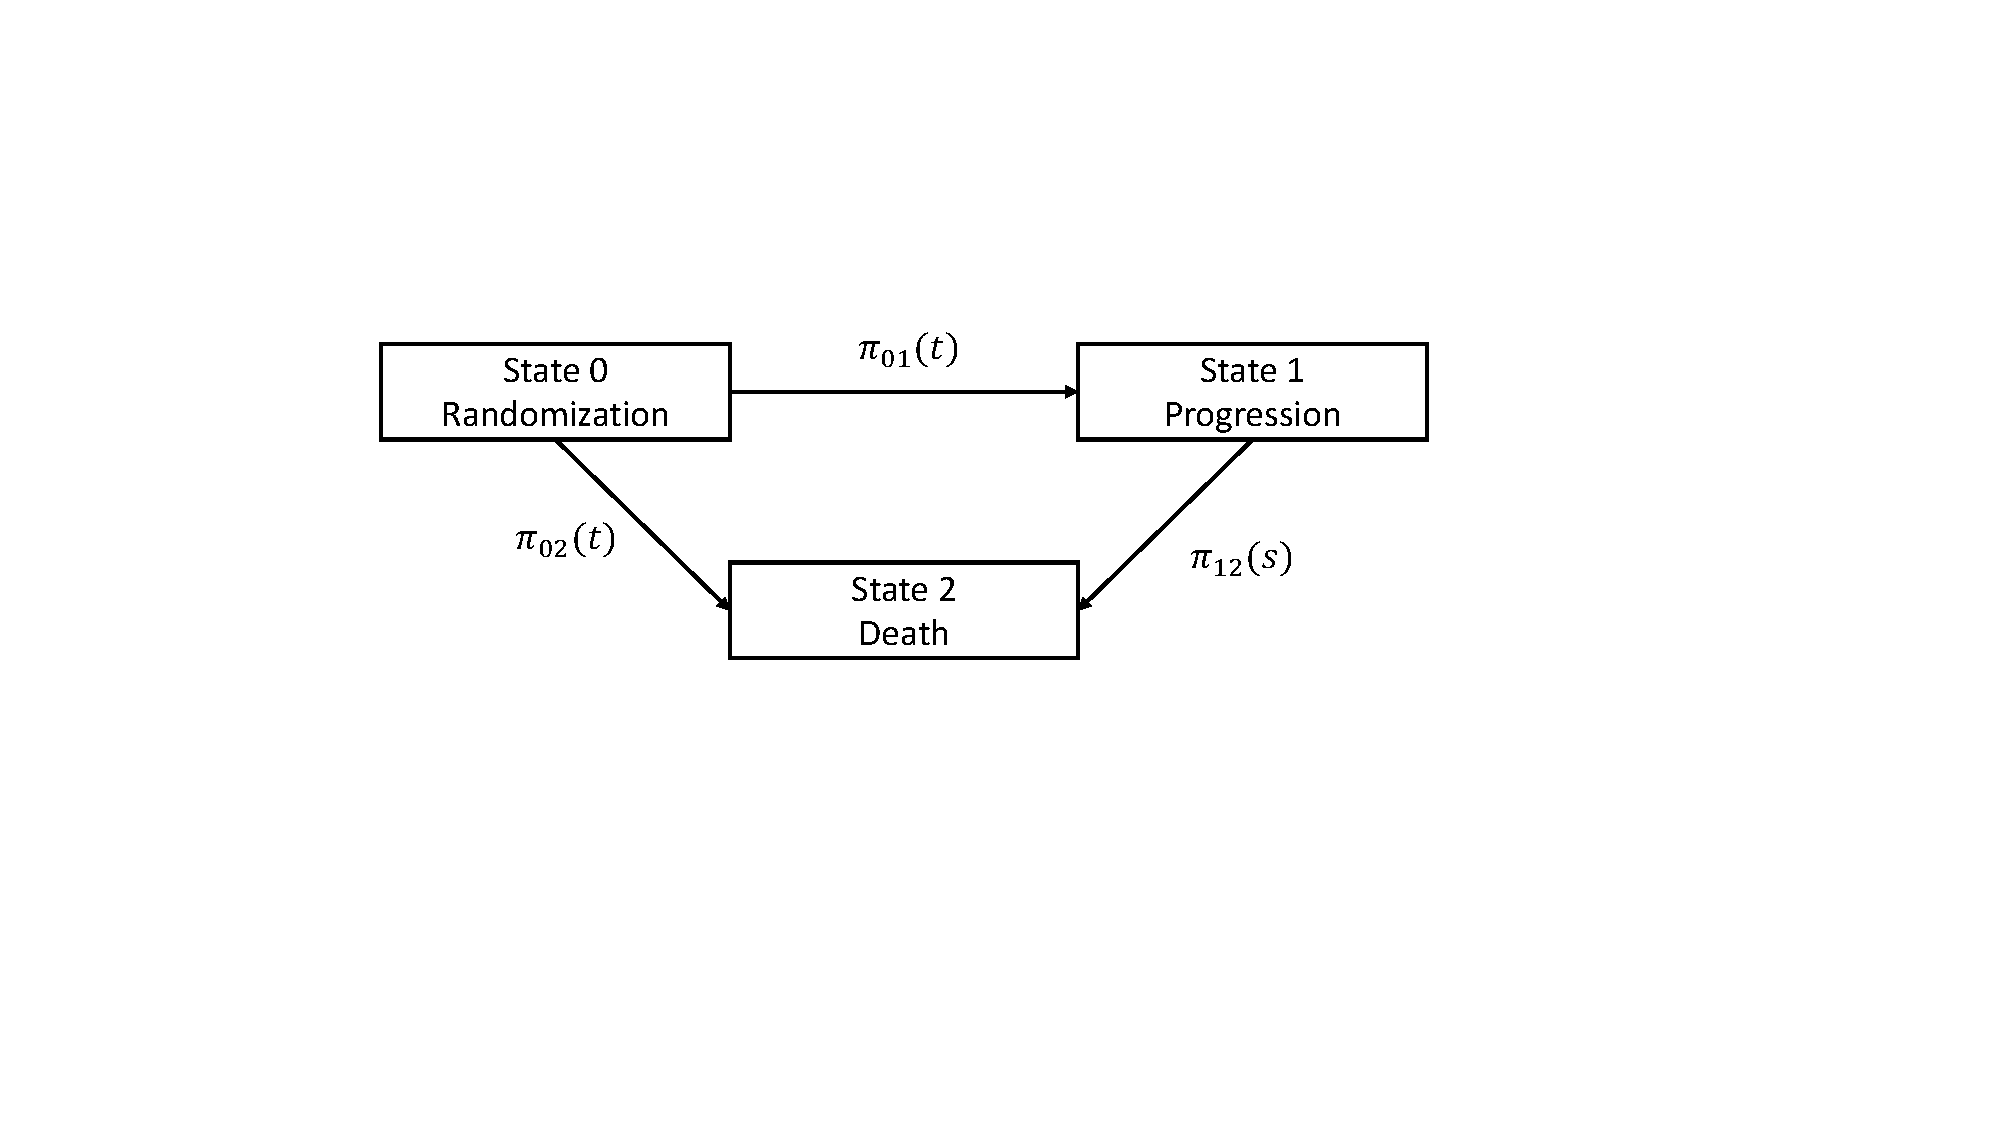
\includegraphics[width=0.7\textwidth]{chapters/figures/multi-state.pdf}
    \caption{The three-state illness-death model \label{fig:multistate}}
\end{figure}

For the illness-death model, transition probabilities represent the probabilities of transition from one state to another over a given time period. Here, we denote the transition probability as $P_{kl}(t_1, t_2)$ from time $t_1$ to $t_2$, where $k$, $l$ describes the state with $k \in {0, 1, 2}$ and $l \in {0, 1, 2}$. The expression of the transition probabilities are given by \citep{meira2009multi}:
$$P_{00}(t_1, t_2) = S_0(t_2 - t_1) = exp{(-\prod_{01}(t_2 - t_1) - \prod_{02}(t_2 - t_1))},$$
$$P_{11}(t_1, t_2) = S_1(t_2 - t_1) = exp{(-\prod_{12}(t_2 - t_1))},$$
$$P_{12}(t_1, t_2) = S_1(t_2 - t_1) = \int_{t_1}^{t_2}P_{11}(t_1, u) \pi_{12}(u;\mathcal{F}_u)P_{22}(u, t_2)du,$$
where $\prod_{kl}(t_1, t_2)=\int_{t_1}^{t_2}\pi_{kl}(t, \mathcal{F}_t)dt$ is the cumulative transition intensity between states $k$ and $l$, where $k \leq l$. If we consider the transition intensities $\pi_{kl}(t; \mathcal{F}_t)$ to follow Weibull distributions, they can be expressed as
$\pi_{01}(t)=\alpha\left(\frac{1}{\gamma_{01}}\right)^\alpha t^{\alpha - 1},$
$\pi_{02}(t)=\alpha\left(\frac{1}{\gamma_{02}}\right)^\alpha t^{\alpha - 1},$
and $\pi_{12}(s)=\alpha\left(\frac{1}{\gamma_{12}}\right)^\alpha s^{\alpha - 1},$
where $\gamma_{01}, \gamma_{02}$ and $\gamma_{03}$ are the scale parameters, $\alpha$ is the shape parameter, $t$ refers to time since randomization and $s$ refers to time since progression. $\gamma_{01}, \gamma_{02}$ and $\gamma_{03}$ for each patient are further defined as $\gamma_{01,i} = \Tilde{\gamma}_{01}exp(\boldsymbol{\beta}_{01}\boldsymbol{X}_i)$, $\gamma_{02,i} = \Tilde{\gamma}_{02}exp(\boldsymbol{\beta}_{02}\boldsymbol{X}_i)$, and $\gamma_{12,i} = \Tilde{\gamma}_{12}exp(\boldsymbol{\beta}_{12}\boldsymbol{X}_i)$, respectively, where $i \in N$, $\boldsymbol{X}_i$ is the vector of covariates, and $\boldsymbol{\beta}_{01}$, $\boldsymbol{\beta}_{02}$ and $\boldsymbol{\beta}_{12}$ are the regression coefficients. The baseline hazards $\Tilde{\gamma}_{01}$, $\Tilde{\gamma}_{02}$, and $\Tilde{\gamma}_{12}$ are estimated using a Weibull distribution. To guarantee the convergence of \ac{MCMC} , a uniform shape parameter $\alpha$ is employed for all three Weibull functions. The multi-state model's likelihood construction is as follows:

Here, we aim to estimate the parameter vector $\theta = (\alpha, \gamma_{01}, \gamma_{02}, \gamma_{12})$ using maximum likelihood estimation. Firstly, we need to model the survival experiences of individuals, which can be characterized by four distinct cases based on a patient's progression through the illness-death model:
1) Patients progress and are then censored,
2) Patients progress and subsequently die,
3) Patients die without prior progression,
4) Patients are censored without experiencing either progression or death. If for every individual \( i \) in the set \( (1, ..., n) \), we let \( t_{i1} \) indicate the duration from the initial state to either progression or death and let \( t_{i2} \), which is conditioned on progression, represents the time from progression to death, then the individual likelihood for these 4 experiences, denoted as \( L_i^{(k)}(\theta) \) where \( k \) varies from 1 to 4, can be described as: $L_i^{(1)}(\theta) = f_1(t_{i1})S_2(t_{i1})S_3(t_{i2})$, $L_i^{(2)}(\theta) = f_1(t_{i1})S_2(t_{i1})f_3(t_{i2})$, $L_i^{(3)}(\theta) = S_1(t_{i1})f_2(t_{i1})$, and $L_i^{(4)}(\theta) = S_1(t_{i1})S_2(t_{i1})$. Here, \( f_1(\cdot) \) and \( S_1(\cdot) \) are density and survival function for time to progression, \( f_2(\cdot) \) and \( S_2(\cdot) \) are density and survival function for time to death without progression, and \( f_3(\cdot) \) and \( S_3(\cdot) \) are density and survival function for time to death post progression. Therefore, comprehensive log-likelihood for all subjects can be formulated as:
\[
\begin{aligned}
\log(L(\theta)) &= \sum_{i=1}^{n}[(d_1)(1-d_2)(1-d_3)L_i^{(1)}(\theta) + (d_1)(1-d_2)(d_3)L_i^{(2)}(\theta) \\
&\quad +(1-d_1)(d_2)L_i^{(3)}(\theta) + (1-d_1)(1-d_2)L_i^{(4)}(\theta)],
\end{aligned}
\]

where \( d_1 \) is the censoring indicator for progression, \( d_2 \) is the indicator for death without preceding progression, and \( d_3 \) is the indicator for death post progression. Note: here, an indicator value of 0 represents censoring, whereas a value of 1 indicates the event's occurrence.


\subsection{Copula Model for Time-to-Progression (TTP) and OS} \label{sec:method_copula}
Similar to the model defined in  \ref{sec:NT}, we use $\lambda_{\rm TTP}(t|\textbf{Z})$ to
denote the hazard function for TTP. Under the Cox
proportional hazards model, we have $\lambda_{\rm TTP}(t|\textbf{Z})=\lambda_{0, \rm TTP}(t)\mathrm{exp}(\textbf{Z}' \boldsymbol{\beta_{\rm TTP}})$, and the corresponding survival function is given by
$S_{\rm TTP}(t|\textbf{Z})=\mathrm{exp}\{-\gamma_{\rm TTP} t^{\alpha_{\rm TTP}}
\mathrm{exp}(\textbf{Z}' \boldsymbol{\beta_{\rm TTP}} )\}$, such that $\gamma_{\rm TTP}$ and $\alpha_{\rm TTP}$ are the scale and shape parameters
of the Weibull distribution, respectively. The Clayton model between \ac{TTP} and \ac{OS} is specified as
\begin{equation*}
S_1(t_{\rm TTP},
t_{\rm OS}|\textbf{Z})=\{S_{\rm TTP}(t_{\rm TTP}|\textbf{Z})^{-\eta_{\rm TTP}}
+S_{\rm OS}(t_{\rm OS}|\textbf{Z})^{-\eta_{\rm TTP}}-1\}^{-1/\eta_{\rm TTP}}, 
\end{equation*}
where $\eta_{\rm TTP}>0$ measures the correlation.
For TTP,
define $y_{\rm TTP}=\mathrm{min}(t_{\rm TTP}, c_{\rm TTP})$ and
$\delta_{\rm TTP}=I(t_{\rm TTP} \le c_{\rm TTP})$,
where $c_{\rm TTP}$ and $I(\cdot)$ denote the censoring time and the indicator function,
respectively; and define $y_{\rm OS}$ and $\delta_{\rm OS}$ similarly for OS. Depending on the censoring pattern, the observed data for the $i$th participant falls into one of the 4 mutually exclusive cases: ($\delta_{TTP}$=1, $\delta_{OS}$=1), ($\delta_{TTP}$=1, $\delta_{OS}$=0),
($\delta_{TTP}$=0, $\delta_{OS}$=1), and ($\delta_{TTP}$=0, $\delta_{OS}$=0).  Figure \ref{fig:copula} illustrates the Clayton copula fitted between \ac{TTP} and OS.

\begin{figure}
\centering
\subfloat[]{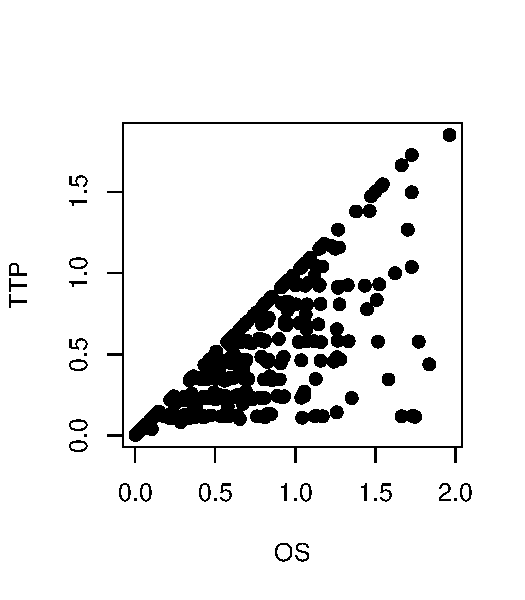
\includegraphics[width=0.31\textwidth]{chapters/figures/scatterplot.pdf}}\label{fig:scatter}
\subfloat[]{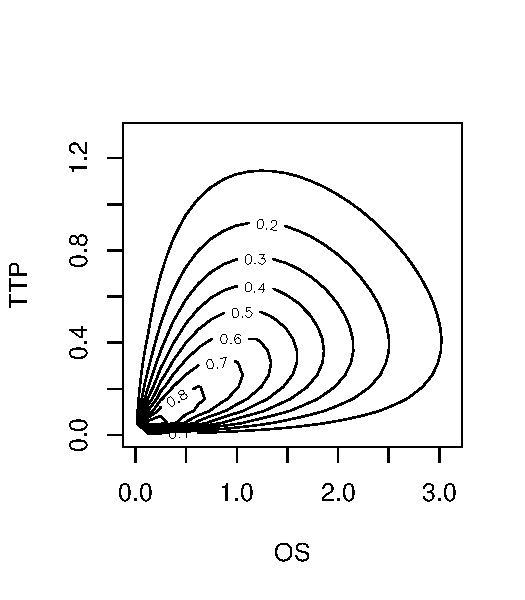
\includegraphics[width=0.325\textwidth]{chapters/figures/contour.pdf}}\label{fig:contour}
\subfloat[]{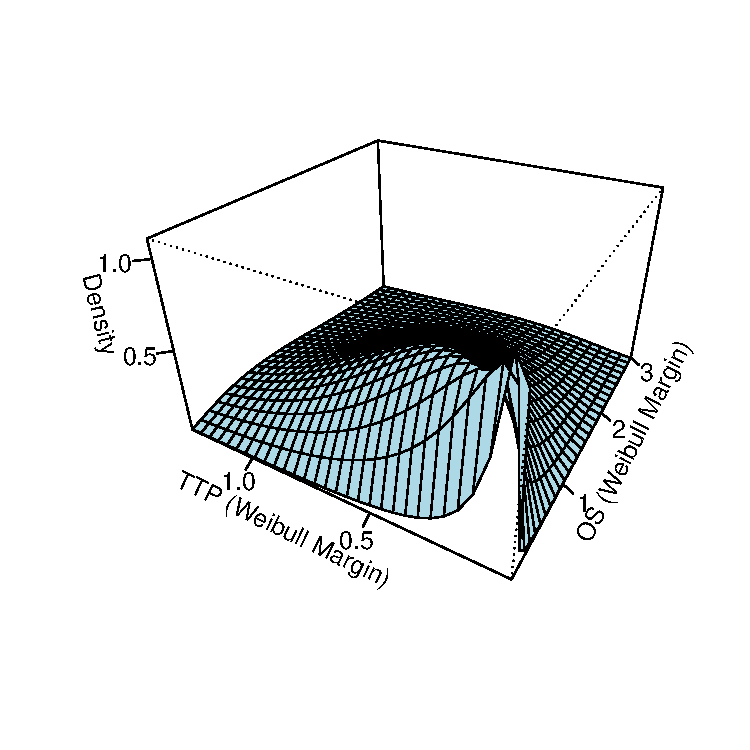
\includegraphics[width=0.35\textwidth]{chapters/figures/surface.pdf}}\label{fig:surface}
\caption{(a) The scatterplot between TTP and OS, (b) the contour plot of TTP vs. OS fitted with a Clayton copula, (c) the surface plot of TTP vs. OS fitted with a Clayton copula. \label{fig:copula}}
\end{figure}

\subsection{Standard Statistical Analysis}\label{sec:method_standard}

Most commonly, \ac{PFS} is modeled using a Kaplan-Meier curve or Cox regression. For example, just like what we discussed previously in Section \ref{sec:marginal}, a simple Weibull baseline hazard model has the form
$\lambda(t)=\alpha \gamma t^{\alpha-1} \exp(\textbf{Z}' \boldsymbol{\beta})$,
where $\textbf{Z}_i$ is the covariate matrix for modeling PFS, $\alpha$ and $\gamma$ are the shape and scale parameters of the Weibull distribution, and $\boldsymbol{\beta}$ is the vector of coefficients. Note that a standard analytic method does not consider the dynamics of the component processes of \ac{PFS} and does not take random effects into account.

\subsection{Prediction}

\subsubsection{Posterior Predictive Distribution (PPD)}
Within each of the models outlined in Sections \ref{sec:method_standard} through \ref{sec:jm}, we utilize the \ac{PPD} technique \citep{gelman2014bayesian} to generate \ac{OS} predictions. The \ac{PPD} represents the distribution of potential unobserved values based on the observed values, and it follows this structure:
$p(y_{pred}|y) = \int{p(y_{pred},\theta|y)d\theta} = \int{p(y_{pred}|\theta,y)p(\theta|y)d\theta} = \int{p(y_{pred}|\theta)p(\theta|y)d\theta}$,
This formulation leverages the conditional independence between $y$ (observed data), $y_{pred}$ (unobserved data), and $\theta$ (parameters). The \ac{PPD} can be understood as an average of conditional predictions over the posterior distribution of $\theta$. During the \ac{MCMC}  process, for each sampled $\theta$ from the posterior distribution, a corresponding $y_{pred}$ sample is obtained. To produce \ac{PPD} samples for \ac{OS} using the survival time modeling methods discussed, we used the \texttt{JAGS} software \citep{plummer2017jags} along with the \texttt{rjags} package for implementation in the R environment.

\subsubsection{Bayesian Model Averaging (BMA)}
In Section \ref{sec:jm}, we have established the three models governing the relationships between the target lesion, non-target lesion, new lesion, and OS, along with the marginal model for \ac{OS} in our joint model, a \ac{BMA} approach can be adopted to link all four models under the multivariate joint modeling approach together, enhancing the overall prediction capability.

In prognostic modeling, it is standard to generate predictions by selecting a single model based on certain metrics. In the context of oncology, different \ac{PFS} components may be more correlated with \ac{OS} under various tumor types or patient groups, thus offering more accurate \ac{OS} predictions. Here, we use \ac{BMA} to calculate the weighted average of the predicted \ac{OS} under the three joint models and one marginal model for \ac{OS} defined above. The weights indicate the plausibility of each model being the most predictive model. We denote the models defined in Section \ref{sec:TL}, \ref{sec:NT}, \ref{sec:NL}, and \ref{sec:marginal} by $M_T$, $M_{NT}$, $M_{NL}$, and $M_{OS}$, respectively. Then by BMA, the final predicted probability of \ac{OS} follows
\begin{align*}
P(Y_{pred}|Data)&=P(Y_{pred.t}|M_T,Data)P(M_T|Data)\\
&+P(Y_{pred.nt}|M_{NT},Data)P(M_{NT}|Data)\\
&+P(Y_{pred.nl}|M_{NL},Data)P(M_{NL}|Data)\\
&+P(Y_{pred.os}|M_{OS},Data)P(M_{OS}|Data),
\end{align*}
where $P(M_T|Data)$, $P(M_{NT}|Data)$, $P(M_{NL}|Data)$, and $P(M_{OS}|Data)$ are the model weights. In general, if we have a total of $Q$ models, the model weight for model $q$ at the $t$th \ac{MCMC}  iteration is  
$$w^{(t)}_q=P(M_q|Data,\theta^{(t)})=\frac{P(M_q,Data,\theta^{(t)})}{P(Data,\theta^{(t)})} =\frac{P(Data|M_q,\theta^{(t)})P(\theta^{(t)}|M_q)P(M_q)}{P(Data,\theta^{(t)})},$$
where $\theta^{(t)} = (\theta_1^{(t)}, \theta_2^{(t)},...,\theta_Q^{(t)})$. If we set $P(\theta_h|M_h, Data)=g_h$, and $q \ne h$, then according to \cite{congdon2007model},
$$P(\theta^{(t)}|M_q)=P(\theta_q^{(t)}|M_q) \prod_{h=1,h\ne q}^Q P(\theta_h^{(t)}|M_q)=P(\theta_q^{(t)}|M_q) \prod_{h=1,h\ne q}^Q g_h.$$
Therefore, 
$$w^{(t)}_q=P(M_q|Data,\theta^{(t)})=\frac{P(Data|M_q,\theta^{(t)}) P(\theta_q^{(t)}|M_q) \prod_{h=1,h\ne q}^Q g_h P(M_q) }{\sum_{k=1}^Q P(Data|M_k,\theta^{(t)}) P(\theta_k^{(t)}|M_k) \prod_{h=1,h\ne k}^K g_h P(M_k)}.
$$
We implement the \ac{BMA} approach using the above formula and calculate the final predicted OS. 



\subsection{Prior Specification}

In this section, we provide recommendations for specifying priors for the parameters in the models discussed in Section \ref{sec:method}. Our aim is to promote the use of generalizable, weakly informative, or non-informative priors for all model parameters to ensure robust and interpretable results. We also emphasize the importance of selecting appropriate priors to maintain parameter identifiability.

\subsubsection{General Guidelines}

For the $\boldsymbol{\beta}$ vector of coefficients, we recommend using weakly informative normal distributions with a mean of 0. We suggest weakly informative exponential distributions for the shape parameters ($\alpha$) in the Weibull distribution. All random effect parameters ($b$) should follow weakly informative normal distributions, denoted as $N(0, \sigma_{b_k}^2)$, where $k$ stands for different random variables under different copula models. Weakly informative half-normal priors are recommended for the standard deviations ($\sigma_{b_k}$) associated with the random effects. For all Clayton copula parameters ($\eta$), we recommend using weakly informative exponential distributions. These priors can accommodate a wide range of plausible values. In the following subsections, we provide recommendations for parameters specific to each model:

\subsubsection{Three-State Illness-Death Model}

In the Three-State Illness-Death Model, we advise using weakly informative half-normal priors for all $\Tilde{\gamma}$ parameters. These priors allow flexibility while constraining extreme values.

\subsubsection{Multivariate Joint Modeling Approach}

In the model assessing the association between target lesion and OS, which is a component of our proposed multivariate joint modeling approach, we suggest the following priors: For the parameter $\lambda$, a weakly informative normal distribution with a mean of 0 is recommended. The correlation coefficient ($\rho$) should have a non-informative prior, such as $Unif(-1, 1)$, to avoid biasing the estimation. Additionally, we assume that all 4 submodels are equally weighted before fitting BMA, that is, $P(M_q) = 1/Q$, for all $q = 1,...,Q$.


\section{Simulation}
\label{sec:simulation}

\subsection{Design}
We performed extensive simulations to evaluate the performance of the proposed multivariate joint modeling approach. All simulated datasets mimic the structure of the renal cell cancer trial data. Specifically, we assume 400 subjects and 25 visits. Longitudinal measurements of target lesion and new lesion status are recorded at each visit. For simplicity purposes, non-target lesion status is not included. Survival status is updated whenever deaths occur. The follow-up visits are scheduled for every two months within the first two years, then change to every three months until the end of the 5th year. We censor the subject's subsequent target lesion measurements and new lesion status whenever that subject's death occurs. In addition, we have assumed three scenarios: 1) \ac{OS} is independent of target lesion measurements and time to new lesion, 2) \ac{OS} is correlated with time to new lesion only, and 3) \ac{OS} is correlated with target lesion measurements only. In all scenarios, target lesion measurements and new lesion status are randomly and independently simulated, but \ac{OS} is generated under different conditions. Specifically, in scenario 1, \ac{OS} is randomly and independently simulated. In scenario 2, \ac{OS} is conditionally simulated from a bivariate copula model between \ac{OS} and new lesion status. Finally, in scenario 3, \ac{OS} is conditionally simulated based on the target lesion measurements. We assume a negative correlation between \ac{OS} and changes in tumor measurements. For each scenario, 100 datasets are generated. To simplify the simulation process, only $treatment$ is included in the covariate matrices. 

We compare predictions under four models: our proposed multivariate joint model (Section \ref{sec:jm}), a copula model for \ac{TTP} and OS (Section \ref{sec:method_copula}), a semi-markov three-state illness-death model \citep{weber2020statistical} (Section \ref{sec:multi-state}), and a marginal Weibull baseline hazard model of OS (Section \ref{sec:method_standard}). 

\begin{figure}
\centering
\subfloat[]{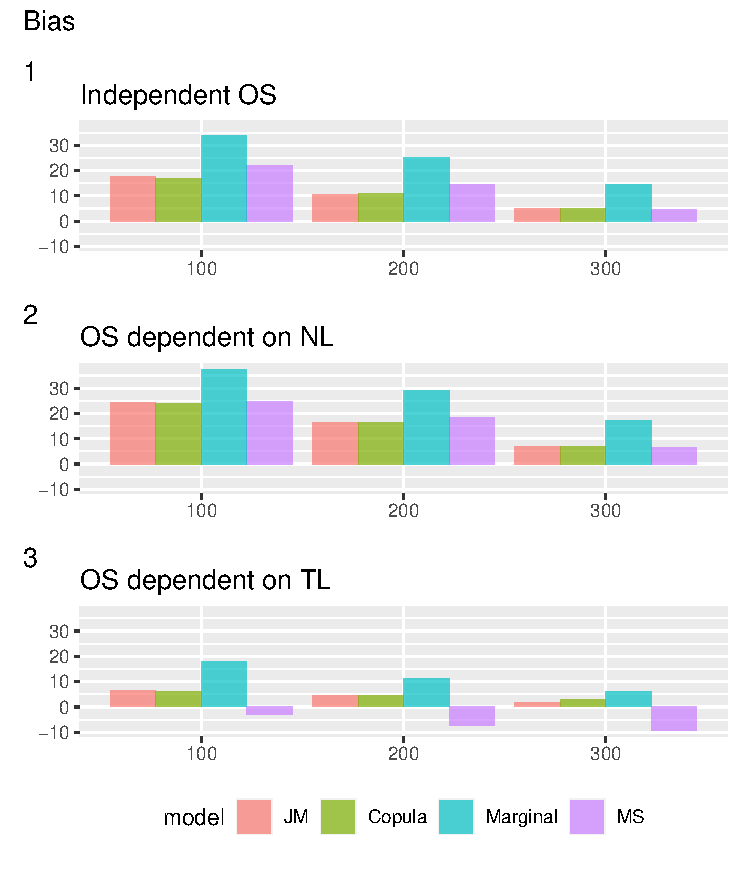
\includegraphics[width=0.5\textwidth]{chapters/figures/Bias.pdf}\label{fig:bias}}
\subfloat[]{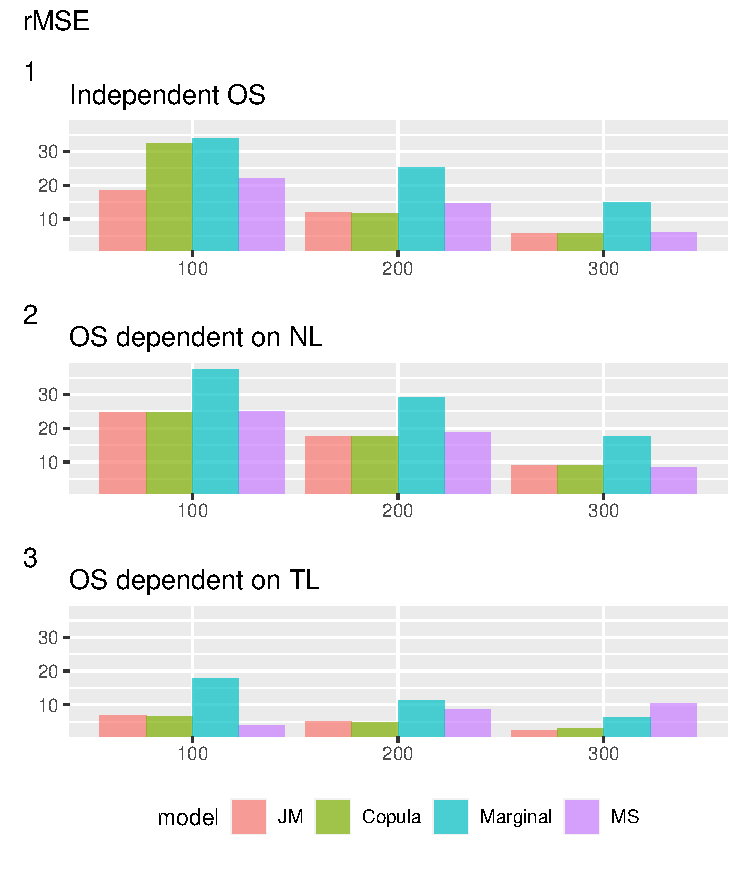
\includegraphics[width=0.5\textwidth]{chapters/figures/rMSE2.pdf}\label{fig:rmse}}
\caption{The bias (a) and rMSE (b) of the last death date predictors of four models: the multivariate joint modeling approach (JM), a copula model between PFS and \ac{OS} (Copula), the marginal Weibull baseline hazard model of OS (Marginal), and a three-state illness-death model (MS), under three OS scenarios. The $x$-axis denotes the number of death at cutoff. The $y$-axis denotes the number of months. \label{fig:result}}
\end{figure}



To emulate real trial scenarios and assess the prediction performance of our proposed method, we generate snapshots of the data such that for each simulated dataset, we have snapshots of what the data would have looked like if only 100, 200, and 300 death events had occurred. Then, we predict the time of the last (400th) death event under each snapshot dataset. Note that predictions may be performed at any time during the trial, and 100, 200, and 300 were selected for illustration purposes. Predictions from the four methods are compared. Finally, we calculate each predictor's \ac{CR}, \ac{rMSE}, bias, and width of the 90\% \ac{CI}. The 90\% \ac{CI} is the narrowest interval that includes 90\% of the posterior distribution of the predictor. 

\subsection{Results}

The bias and \ac{rMSE} of the predicted time of the last death are shown in Figures \ref{fig:bias} and \ref{fig:rmse}, and the corresponding \ac{CR} and \ac{CI} width are shown in Table \ref{tab:sim_result}. The weights of all submodels of the multivariate joint modeling approach under each simulation scenario are shown in Figure \ref{fig:weights_simulation}.

\begin{table}
\caption{The coverage rate (CR) and credible interval (CI) width for predictors of the time of the last death. Comparing the results from the multivariate joint modeling approach (JM), a copula model between PFS and OS (Cop), a three-state illness-death model (MS), and the marginal Weibull baseline hazard model of OS (Mrgl). The unit for CI width is month.  \label{tab:sim_result}}
\begin{center}
\begin{tabular}{ccccccccccccc}
& \multicolumn{4}{c}{Independent OS} & \multicolumn{4}{c}{OS dependent on NL} & \multicolumn{4}{c}{OS dependent on TL} \\ 
& JM & Cop & MS & Mrgl & JM & Cop & MS & Mrgl & JM & Cop & MS & Mrgl \\ \hline
\multicolumn{10}{l}{\textit{100 death event}}\\
CR & 0.49 & 0.49 & 0.01 & 0.00 & 0.11 & 0.11 & 0.03 & 0.00 &  0.91 & 0.91 & 1.00 & 0.00 \\ 
Width & 35.9 & 35.8 & 24.9 & 3.4  & 29.2 & 29.5 & 26.8 & 2.9  &  24.4 & 25.4 & 41.8 & 3.2 \\ \hline
\multicolumn{10}{l}{\textit{200 death event}}\\
CR & 0.89 & 0.86 & 0.33 & 0.00 & 0.45 & 0.45 & 0.24 & 0.00 & 0.85 & 0.98 & 1.00 & 0.00 \\ 
Width & 35.7 & 35.3 & 26.0 & 5.9 & 32.2 & 32.2 & 26.8 & 5.6 & 15.2 & 17.1 & 39.6 & 4.1  \\ \hline
\multicolumn{10}{l}{\textit{300 death event}}\\
CR & 0.98 & 0.98 & 0.98 & 0.00 & 0.90 & 0.89 &  0.95 & 0.01  & 0.97 & 0.98 & 1.00 & 0.00 \\ 
Width & 30.5 & 30.5 & 29.6 & 9.3 & 32.5 & 32.6 & 31.5 & 9.9 & 12.0 & 11.2 & 36.7 & 4.6 \\ 
\hline
\end{tabular}
\end{center}
\end{table}


\begin{figure}
\centering
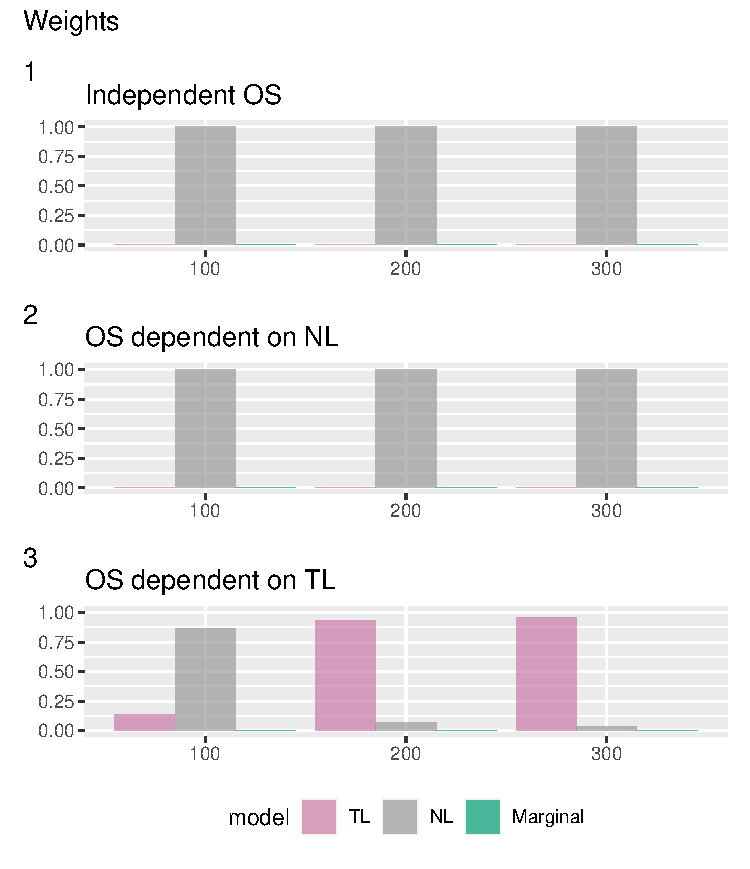
\includegraphics[width=8cm]{chapters/figures/Weights_simulation.pdf}
\caption{The weights of all submodels of the multivariate joint modeling approach for each snapshot dataset in the simulation studies.\label{fig:weights_simulation}}
\end{figure}

Under scenario 1, where \ac{OS} is generated independently, the bias and \ac{rMSE} of all predictors become smaller as we gather more information from the trial, i.e., more death events are observed. Overall, the marginal model performs worse than the other three models. This is likely due to the conservativeness of the Weibull model and the fact that it only utilizes \ac{OS} data, causing predictions to concentrate near the observed maximum OS. Given that the proposed model assigned all the weight to the copula model between new lesion and OS, it is reasonable that the copula model and the multivariate joint modeling approach have similar bias and \ac{rMSE}. Having evaluated all the metrics, the multivariate joint modeling approach and the copula model are the best-performing method under scenario 1.

In Scenario 2, where \ac{OS} is generated based on new lesion status, the multivariate joint modeling approach, the copula model, and the three-state illness-death model exhibit similar bias and \ac{rMSE} values. Once again, the marginal model lags behind the other models in performance. As with Scenario 1, as the number of observed death events increases, the bias and \ac{rMSE} of all predictors decrease. Compared to Scenario 1, the improved performance in bias and \ac{rMSE} of the three-state illness-death model can largely be attributed to the fact that the \ac{OS} observations generated under Scenario 2 more closely resemble a Weibull distribution. However, when only 100 or 200 death events are observed, the three-state illness-death model has a lower \ac{CR} than the other two. This might be due to the conservatives of the standard Weibull model. Consequently, for Scenario 2, we would still recommend either the joint modeling approach or the copula model.

In Scenario 3, where \ac{OS} is derived based on target lesion measurements, the proposed multivariate joint modeling approach begins to surpass the copula model as more death events are observed. Simultaneously, as the count of observed death events increases, the multivariate joint modeling approach assigns greater weight to the joint model between the target lesion and OS, which is anticipated. This is expected as the multivariate joint modeling approach is the only method that captures the relationship between \ac{OS} and the target lesion. Differing from the other two scenarios, the bias and \ac{rMSE} of predictors from the three-state illness-death model do not consistently diminish with the increase in observed death events. Moreover, the three-state model displays the widest \ac{CI} among all the models. This can be attributed to the alteration in \ac{OS} distributions, as it is generated based on the target lesion distribution, which does not conform to a Weibull distribution. The inflexibility of the standard Weibull baseline hazard model, devoid of random effects, further contributes to this.

According to Figure \ref{fig:result}, across all scenarios, the proposed multivariate joint modeling approach performs either the best or very similar to the copula model, if the copula model is the best-performing one. This is reasonable as the \ac{BMA} could assign $w_q = 1$ to submodel $q$ when submodel $q$ is significantly better than the other $q-1$ submodels. If this is the case, the multivariate joint modeling approach predictions will be the same as the predictions from its submodel $q$. The multivariate joint modeling approach and the copula model are less sensitive to changes in the \ac{OS} distribution and still provide relatively reasonable predictions even when \ac{OS} prediction does not closely resemble a Weibull distribution. In summary, the multivariate joint modeling approach provides the most reliable predictions across all tested scenarios.

\begin{figure}
\centering
\subfloat[]
{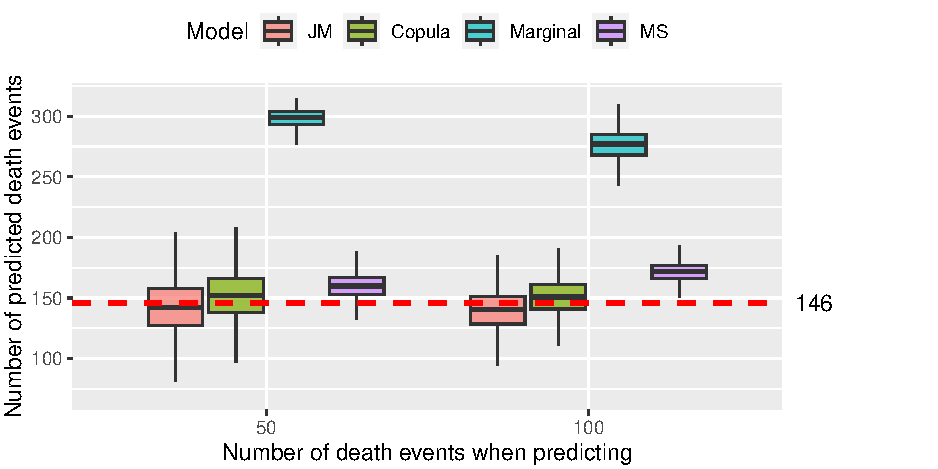
\includegraphics[width=0.74\textwidth]{chapters/figures/primary_analysis.pdf}\label{fig:primaryanalysis}}
\hfill
\subfloat[]
{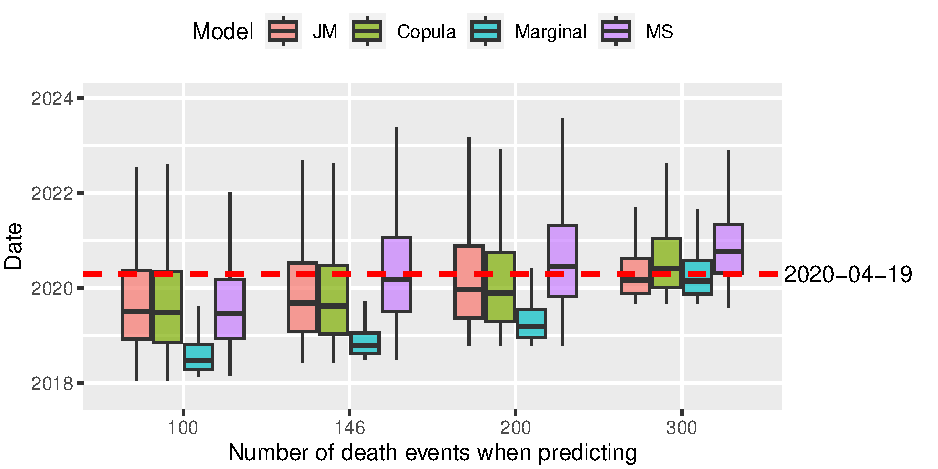
\includegraphics[width=0.74\textwidth]{chapters/figures/lastdeath1.pdf}\label{fig:casestudy}}
\hfill
\subfloat[]
{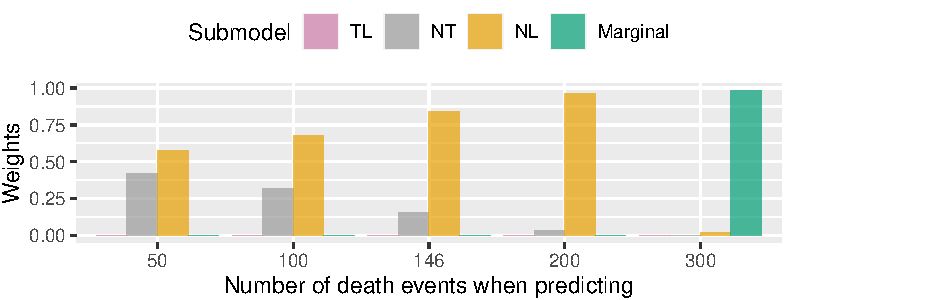
\includegraphics[width=0.74\textwidth]{chapters/figures/weights.pdf}\label{fig:weights}}
\caption{(a) Boxplots of the posterior distributions of the last death date by the proposed multivariate joint modeling approach, the copula model between PFS and OS, the marginal Weibull baseline hazard model of OS, and the three-state illness-death model. Date ``2020-04-19" is the true last death date. (b) The final weights of each submodel under the proposed multivariate joint modeling approach. (c) The weights of all submodels of the multivariate joint modeling approach for each recreated dataset.}
\end{figure}

\section{Analysis of the Renal Cell Carcinoma Data}
\label{sec:caseanalysis}
We return to the renal cell carcinoma dataset introduced in Section \ref{sec:example}. Our objective here is to predict the timing of the last death in this clinical trial by fitting the multivariate joint model we developed in Section \ref{sec:jm} to all available tumor measurements. We generate snapshots of the trial data at the 100th, 146th (the time of primary analysis), 200th, and 300th death, and compare predictions under four models: the multivariate joint model, a copula model for \ac{TTP} and OS, a three-state illness-death model, and a marginal model of OS. 

We included \textit{gender, age, nephrectomy at baseline, Heng prognostic criteria at baseline, and ECOG Performance Status} into the covariates matrix $\textbf{X}_i$ and $\textbf{Z}_i$. Then, we fit each model using two \ac{MCMC}  chains, each with at least 10,000 \ac{MCMC}  iterations, 1,000 burn-in, and 8,000 adaptation iterations.  Convergence diagnostic tests and autocorrelation plots did not show any alarming indications of convergence failure. Figure \ref{fig:primaryanalysis} displays the predicted number of deaths at the time of the primary analysis. Figure \ref{fig:casestudy} presents boxplots of the posterior distributions for the predictors of the last death date from all tested models compared to the true last death date. The median values of the boxplots serve as point predictions. Figure \ref{fig:weights} displays the weights of all submodels for each recreated dataset. In this specific case study, the new lesion is observed to have the strongest correlation with OS. Therefore, it makes sense that greater weights are assigned to the new lesion copula submodel, and the copula model between \ac{TTP} and \ac{OS} also performs well. While the marginal model exhibits significantly smaller \ac{CI}s, its predictors prove to be less accurate than those of the multivariate joint modeling approach and the copula model, especially when we observe 100, 146, and 200 deaths. These latter models consistently demonstrate the most reliable performance improvements as the number of observed deaths increases. When we have 300 deaths observed and the marginal model performs the best among all submodels, the \ac{BMA} procedure naturally assigns more weight to it, as indicated in Figures \ref{fig:casestudy} and \ref{fig:weights}. Considering that the posterior samples of the three-state illness-death model are derived by combining predictions from two distinct time periods - randomization to progression and progression to death — it is reasonable for the three-state model to exhibit the widest \ac{CI}s. 

\begin{table}
\caption{Bias and \ac{rMSE} of the predictors of multivariate joint modeling approach (JM), copula model, marginal model, and three-state illness-death model (MS). \label{tab:casestudytable}}
\begin{center}
\begin{tabular}{ccccccc}
\hline
\multicolumn{2}{c}{No. of events} & \multirow{2}{*}{Metric} & \multirow{2}{*}{JM} & \multirow{2}{*}{Copula} & \multirow{2}{*}{Marginal} & \multirow{2}{*}{MS}\\ 
Observed & Predicted & & & & & \\\hline
\multirow{2}{*}{100} & \multirow{2}{*}{241} & Bias & 0.67 & 1.71 & 9.46 & 1.35\\
&& rMSE & 3.71 & 3.94 & 10.56 & 3.73 \\ \hline
\multirow{2}{*}{146} & \multirow{2}{*}{195} & Bias & 1.41 & 2.11 & 9.13 & 2.54\\
&& rMSE & 2.56 & 3.13 & 9.65 & 3.14 \\ \hline
\multirow{2}{*}{200} & \multirow{2}{*}{141} & Bias & 0.91 & 2.15 & 7.89 & 3.11\\
&& rMSE & 2.06 & 2.91 & 8.19 & 3.65 \\ \hline
\multirow{2}{*}{300} & \multirow{2}{*}{41} & Bias & 6.23 & 2.97 & 6.32 & 4.13  \\
&& rMSE & 8.24 & 6.14 & 8.28 & 7.31  \\ \hline
\end{tabular}
\end{center}
\end{table}

Table \ref{tab:casestudytable} presents the bias and \ac{rMSE} of the predicted \ac{OS} when 100, 146, 200, or 300 death events are observed. In the first three scenarios, the multivariate joint modeling approach performs similarly to the copula model and the three-state model. In the last scenario, the joint model performs similarly to the marginal model, consistent with the submodel weights shown in Figure \ref{fig:weights}. Additionally, the joint model exhibits smaller bias and rMSEs compared to the marginal model under all scenarios. While the multivariate joint modeling approach may not always have the smallest bias in this particular case study dataset, its prediction reliability is consistently verified. 

We used all four models to forecast the \ac{OS} of patients with censored \ac{OS} in the case study data set. Subsequently, we generated predicted Kaplan-Meier plots for each model (Figure \ref{fig:predictionKM}). Finally, we estimated the potential gain or loss in life expectancy by calculating the difference in the area under the curve between the experimental drug and the standard of care \citep{pak2017interpretability, survRM2}. The results from Figure \ref{fig:predictionKM} indicate that all models consistently project a substantial improvement in life years. In addition, the multivariate joint modeling approach and the copula model, whose reliability was previously established in this case study, both forecast a roughly 7.5-month gain in life years for patients who receive the experimental drug, as opposed to the standard of care.


\section{Discussion}
\label{sec:discussion}
In this paper, we were motivated by an advanced renal cell carcinoma clinical trial to present how real-time \ac{OS} predictions from joint models with different components of \ac{PFS} can be dynamically combined via BMA. This multivariate joint modeling approach provides reliable estimates of the time of the $n$th death in a trial using all available tumor assessment data based on \ac{RECIST} 1.1. This is valuable for clinical trial planning and patients' end-of-life medical care. Furthermore, the proposed multivariate joint model method provides the most reliable and robust predictions in the case study and across all the scenarios we tested in the simulation studies. This approach can be easily applied to other solid tumor types beyond renal cell carcinoma.

\begin{figure}[H]
    \centering
    \subfloat[]{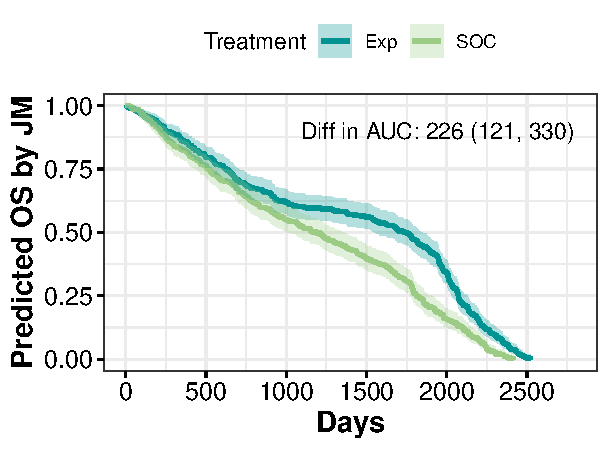
\includegraphics[width=0.49\textwidth]{chapters/figures/JMprediction.pdf}\label{fig:JMprediction}}
    \subfloat[]
    {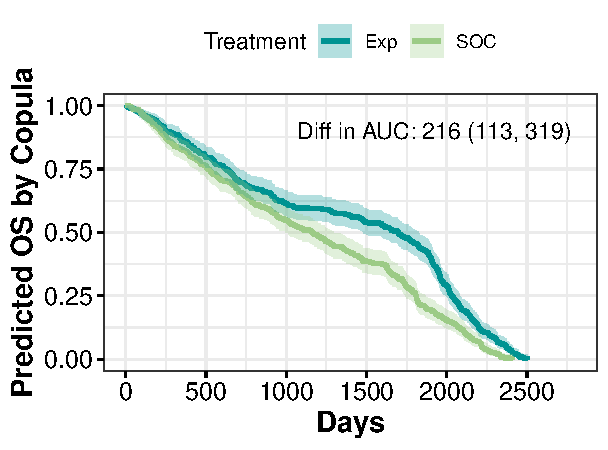
\includegraphics[width=0.49\textwidth]{chapters/figures/copulaprediction.pdf}\label{fig:Copulaprediction}}
    \hfill
    \subfloat[]{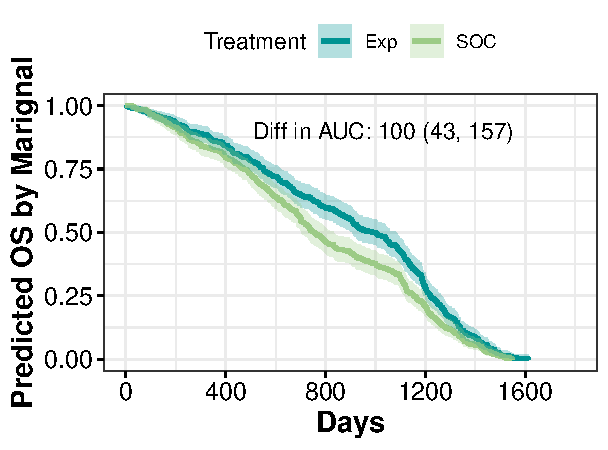
\includegraphics[width=0.49\textwidth]{chapters/figures/marginalprediction.pdf}\label{fig:Marginalprediction}}
    \subfloat[]{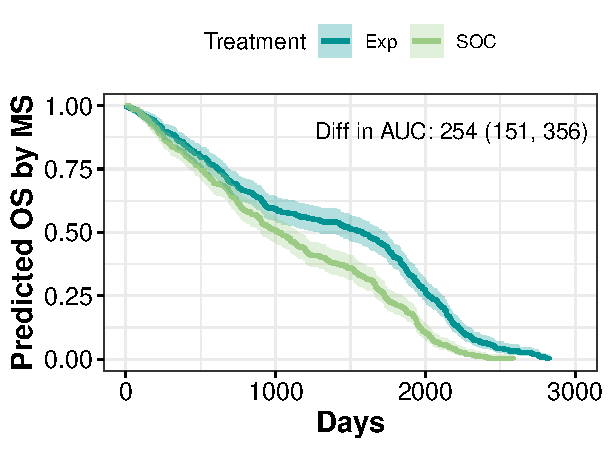
\includegraphics[width=0.49\textwidth]{chapters/figures/MSprediction.pdf}\label{fig:MSprediction}}
    \caption{Kaplan-Meier plots of the observed and predicted overall survival by the multivariate joint modeling approach (a), the copula model(b), the marginal model (c), and the three-state illness-death model. The difference in the area under the curve (AUC) and its CIs for the experimental drug (Exp) and the standard of care (SOC) are also included.}
    \label{fig:predictionKM}
\end{figure}

The multivariate joint modeling approach is flexible and can easily incorporate a linear model with time-dependent covariates or a nonlinear mixed-effects model. Although \ac{BMA} methods optimally combine multiple models, they typically require extended training time due to their complexity. In the example data analysis, only five covariates were included. Incorporating additional baseline characteristics is possible, but doing so would expand the covariate matrix and further increase the computational demands of the multivariate joint modeling approach. Considering that the covariates utilized in each submodel may vary, it is beneficial to determine the most suitable covariates for each submodel before implementation. This covariates selection process can be guided by expert opinion or variable selection models, potentially reducing the covariate matrix's size.

Based on the simulation studies and the example data analysis, it is evident that the copula model for \ac{TTP} and \ac{OS} ranks as the second most reliable model among all those tested. If the \ac{TTP} and \ac{OS} data are well-fitted by Weibull distributions with random effects, the copula model typically performs better than the marginal \ac{OS} model. Therefore, fitting only a copula model with random effects is an excellent option to reduce model training time. Based on our simulations, without including random effects, high variability between individuals will cause the copula model's predictions to be too heavy-tailed.

For a marginal \ac{OS} model to perform better, it would be beneficial to incorporate more predictive covariates or use a model offering greater flexibility than the Weibull baseline hazard model, such as parametric regression models. Similarly, to improve the performance of the multi-state model, we could replace the Weibull baseline hazard model with more flexible models.

During the simulation studies, the data for non-target lesions was not simulated, yet it was included in the example data analysis. This does not undermine the outcome of our simulation studies, given that both the non-target lesion and new lesion were modeled using the exact same joint model, and each component of \ac{PFS} was modeled separately. If the non-target lesion data had been included in the simulation dataset, we would anticipate longer training times for the multivariate joint modeling approach without observing any relative improvement in performance given the scenarios we defined.

Apart from applying the same model weights for all the patients in the dataset, \ac{BMA} can potentially provide personalized model weights, i.e., for different patients, different models may have higher weights. This could further improve the prediction accuracy. Future work can explore how to implement personalized model weights in a time-efficient manner under the setting of this study.